%% When is product of Z_n groups cyclic. I have begun writing this below.

%%%%(c)
%%%%(c)  This file is a portion of the source for the textbook
%%%%(c)
%%%%(c)    Abstract Algebra: Theory and Applications
%%%%(c)    Copyright 1997 by Thomas W. Judson
%%%%(c)
%%%%(c)  See the file COPYING.txt for copying conditions
%%%%(c)
%%%%(c)

\chap{Introduction to Groups\quad
\sectionvideohref{IvNQQuG2ngY&list=PL2uooHqQ6T7PW5na4EX8rQX2WvBBdM8Qo&index=25}}{groups}


\begin{quote}
``There are more groups in heaven and earth, Horatio, than are dreamt of in your philosophy.'' Shakespeare, \emph{Hamlet}, Act 1 Scene V (paraphrase by J. Hill)
\end{quote}

\begin{quote}
``Groups tend to be more extreme than individuals.'' (Daniel Kahneman, 2002 Nobel Prize winner in Economics)
\end{quote}

\begin{quote}
``I am rarely bored alone; I am often bored in groups.'' (Dr. Laurie Helgoe, psychologist)
\end{quote}

You may have noticed that we have been voyaging deeper and deeper into unfamiliar mathematical territory. We're using more symbols and fewer numbers. We introduce unfamiliar terminology and strange notation. We deal with outlandish mathematical objects that are harder and harder to visualize. 

Please rest assured that these elaborations have a practical purpose\footnote{(that is, besides tormenting math students)}. We live in a complicated world, and complicated mathematical structures are needed to describe it well. However, underlying this confusing tangle of complicated structures are some deep commonalities. The purpose of abstraction is to identify and characterize these commonalities. In this way we can make connections between very different fields of mathematics, and gain a much more holistic view of how things work together.
 
One of the commonalities that we have been (more or less) subtly emphasizing in the previous chapters is the ubiquity of \emph{groups}, together with related notions such as isomorphisms and subgroups. Now that you've studies several specific groups (such as ${\mathbb C}, {\mathbb Z}_n, D_n, S_n, A_n$ and so on) our hope is that from these examples you've begun to get a feel for how groups work, and how one should think about groups in general. In this chapter, we will study groups \emph{in the abstract}: that is, we will describe properties that are common to \emph{all} groups, whether finite or infinite, commutative (abelian) or non-abelian, and so on.
\medskip

Thanks to Tom Judson for material used in this chapter.

%What you've seen of groups is only the very beginning. There are groups (and applications of groups) that are almost unimaginably bizarre. To paraphrase Shakespeare:  ``There are more groups in heaven and earth, Horatio, than are dreamt of in your philosophy.''\footnote{Hamlet, Act 1 Scene V.} But no matter how bizarre, all of these groups must obey the fundamental properties of groups -- which is why we now turn to study groups in the abstract.  
% In the last chapter we turned a corner in our study of abstract algebra.  In Chapters~\ref{complex} through \ref{symmetries} we did lots of "regular" algebra, that is, we represented various numbers with variables, and manipulated equations with these variables.  We then took those variables and organized them into sets, functions, groups, Cayley tables, etc.; into generalized structures.  Some of this was not what you had seen in Algebra before, but it wasn't a stretch to come up with or hard to understand based on the algebra you know.  It was simply representing the world with variables.   But in Permutations we started the real stretch that turns regular algebra into abstract algebra.  We took those variables and structures and started to generalize \emph{them}; we started to generalize our structures, our groups, into even more general representations.  In the process we also generalized concepts:  isomorphic groups are like equivalent elements; subgroups are like subsets; the order of a set has an analogous meaning to that of absolute value.
% It is this process of generalizing generalizations that is the crux of studying and thinking Abstract Algebra.  Because if we can generalize a structure or concept to its highest point, and then discover some property about that generalization, then all examples that fit that generalization have to have that same property.  Therefore instead of deeply studying multitudes of different phenomena and contexts in our world and seeing how their parts interact, if we can show that those phenomena and parts fit a generalization, then we know immediately that all properties of that group will show up in that phenomena and the interaction of its parts.  We can deductively know things about the order and operation of this universe without having to inductively test and rigorously prove a theory.  

%Abstract Algebra is logic and Algebra on steroids. 
%So let's generalize our first generalization:  Groups.

\section{Formal definition of a group}\label{groups_section_define}

Historically, the theory of groups first arose from attempts to find the roots of polynomials in terms of their coefficients.  But groups have moved far beyond their original application, and now play a central role in such areas as coding theory, counting, and the study of  symmetries. Many areas of biology, chemistry, and physics have benefited from group theory. In the preceding chapters we've already worked with a number of different groups, including the integers mod $n$ and the symmetries of a rectangle or regular polygon. Recall that a group basically consists of a set and a ``compatible'' operation:

\begin{exercise}{}
\begin{enumerate}[(a)]
\item
What operation is the set ${\mathbb Z}_n$ a group under?
\item
What operation is the set $S_3$ a group under?
\end{enumerate}
\end{exercise}
The following definition formalizes the notion of ``operation''.

\begin{defn} \label{group_op}
 A \term{binary operation}\index{Binary!operation}\index{Operation!binary} or \term{law of composition}\index{Composition!law of}\index{Operation!binary} on a set $G$ is a function $G \times G \rightarrow G$ that assigns to each pair $(a,b) \in G \times G$ a unique element $a \circ b$, or $ab$ in $G$, called the \term{composition} of $a$ and $b$.
\end{defn}

\begin{rem}
\begin{itemize}
\item
Notice that the word ''composition'' is now used to denote any operation on the elements of a set, and not just composition of functions.
\item
When the law of composition on a set is a basic algebraic operation such as multiplication or addition, we'll call it with its usual name.  When it isn't, we will often refer to $a \circ b$  as the ``product'' of $a$ and $b$  (as we did in the Permutations chapter).
\end{itemize}
\end{rem}

In the Modular Arithmetic chapter we introduced what properties a set and operation must have to be called a group:

\begin{exercise}{group_prop}
What are the four properties a set $G$ and a binary operation must exhibit in order for the set to be a group under that binary operation?
\end{exercise}
Building on our previous discussion, we now  proudly present the following formal definition.

\begin{defn}\label{group_definition}
 A \term{group}\index{Group!definition} $(G, \circ )$ is a set $G$ together with a law of composition $(a,b) \mapsto a \circ b$ that satisfies the following axioms. 
\begin{enumerate}
\item
The set $G$ is \term{closed} under the law of composition.  That is, 
\[
\forall a,b \in G, a \circ b = c \mbox{ for some } c \in G .
\]
\item
There exists an element $e \in G$, called the \term{identity element}\index{Element!identity}\index{Identity!element}, such that for any element $a \in G$ 
\[
e \circ a = a \circ e = a.
\]
\item
For each element $a \in G$, there exists an \term{inverse element}\index{Element!inverse}\index{Inverse!element} in G, denoted by $a^{-1}$, such that 
\[
a \circ a^{-1} = a^{-1} \circ a = e.
\]
\item
The law of composition is \term{associative}. That is,
\[
(a \circ b) \circ c = a \circ (b \circ c)
\]
for $a, b, c \in G$.
 
\end{enumerate}
\end{defn}

\begin{rem}
When the group operation is obvious or has been previously specified, we may denote the group by $G$ rather than $(G,\circ)$.  For instance, the group of integers under addition is typically denoted by ${\mathbb Z}$ and not $({\mathbb Z},+)$, since the operation $+$ is understood. 
\end{rem}

One very important class of groups is the commutative groups, which are given their own special designation:

\begin{defn} \label{abelian_group} 
A group $(G,\circ)$ with the property that $a \circ b = b \circ a$ for all $a, b \in G$ is called \term{abelian}\index{Abelian group}\index{Group!abelian}\footnote{In honor of Neils Henrik Abel (1802-1829), an astounding mathematician who sadly died very young of tuberculosis. There is some discussion among mathematicians over whether `abelian' should be capitalized. The word has become so common in mathematics that it's usually treated as a regular word and not a proper name. This should be considered as a special honor to Abel, since his name has become part of the fundamental language of mathematics.}  or \term{commutative}\index{Group!commutative}.  Groups not satisfying this property are said to be  \term{non-abelian}\index{Group!non-abelian} or \term{noncommutative}\index{Group!noncommutative}. 
\end{defn}

Finally, based on our discussion before about the order of sets, we have:

\begin{defn} \label{group_order}
A group is \term{finite}\index{Group!finite}, or has \term{finite
order}, if it contains a finite number of elements The \term*{order}\index{Group!order of}\index{Order!of a group}
of a finite group is the number of elements that it contains. If $G$
is a group containing $n$ elements, we write $|G| =
n$. A group that is not finite is called \term{infinite}, and such a group is said to be of \term{infinite
order}\index{Group!infinite}.
\end{defn} 

The group ${\mathbb Z}_5$ is a finite group of order
5, so $|{\mathbb Z}|_5=5$; while the integers ${\mathbb Z}$ form an infinite group under addition, and
we sometimes write $|{\mathbb Z}| = \infty$.

\begin{defn} \label{trivial_group}
The \term{trivial group}\index{Group!trivial}, consists of the single element $e$  (or ${\var id}$, in our previous notation).
\end{defn} 

\begin{exercise}{trivial}
Prove that the trivial group is in fact a group according to Definition~\ref{group_definition}.
\end{exercise}

\section{Examples}\label{Examples}

There are multitudes upon multitudes of groups besides those we've seen so far.  Some are modifications of groups we are very familiar with.  

\begin{example}{Rstar_group}
The set ${\mathbb R} \setminus \{0 \}$ of non-zero real numbers is written as ${\mathbb R}^{\ast}$.  Let's prove that $({\mathbb R}^{\ast}, \cdot)$ is a group.
\begin{enumerate}[(1)]
\item
Closure:  

\noindent
Suppose $a, b \in {\mathbb R}^{\ast}$.  Then to prove closure we must show $ab \in {\mathbb R}^{\ast}$; that is, we must show (i)
$ab \in {\mathbb R}$ and (ii) $ab \neq 0$:

\medskip{}
\noindent
(i):  Since $a, b \in {\mathbb R}$, and we know ${\mathbb R}$ is closed under multiplication, then $ab \in {\mathbb R}$.

\medskip{}
\noindent
(ii):  Suppose $ab = 0$.  Then as we  noted in Section~\ref{OpsAndRels}, we know either $a = 0$ or $b = 0$.  But $a, b \in {\mathbb R}^{\ast}$; i.e. $a, b \neq 0$.  So we have a contradiction.  Hence $ab \neq 0$.

\medskip{}
\noindent
Therefore $ab \in {\mathbb R}^{\ast}$; and so ${\mathbb R}^{\ast}$  is closed under multiplication.
\end{enumerate}
To finish the proof that ${\mathbb R}^{\ast}$ is a group, we must establish axioms (2) through (4) in Definition~\ref{group_definition}. We leave this up to you in the following exercise:

\begin{exercise}{Rstar_group} 
\begin{enumerate}[(a)]
\item
Finish proving that $({\mathbb R}^{\ast}, \cdot)$ is a group.
\item
Either prove or disprove that $({\mathbb R}^{\ast}, +)$ is a group.
\item
What is the order of $({\mathbb R}^{\ast}, \cdot)$?
\end{enumerate}
\end{exercise}
  \end{example}


\begin{exercise}{C_star}
Let ${\mathbb C}^{\ast} $\label{noteCstar} be the set of non-zero complex 
numbers. 
\begin{enumerate}[(a)]
\item
Why is ${\mathbb C}^{\ast}$ not a group under the operation of complex addition?
\item
Prove ${\mathbb C}^{\ast}$ is a group under the operation of (complex) multiplication.
\item
What is $| ({\mathbb C}^{\ast}, \cdot) |$?
\item
Is $({\mathbb C}^{\ast}, \cdot)$ an abelian group?  Justify your answer.
\end{enumerate}  
\end{exercise}

\begin{rem}
Groups based on sets of numbers that \emph{include} 0 (such as ${\mathbb R}, {\mathbb C}, {\mathbb Q}$) are assumed to have the group operation $+$ (unless otherwise stated). For groups based on sets of numbers that \emph{exclude} $0$ such as ${\mathbb R^\ast}, {\mathbb C^\ast}, {\mathbb Q^\ast}$, the group operation is assumed to be multiplication (unless otherwise stated).
\end{rem}
 
\begin{exercise}{15}
\begin{enumerate}[(a)]
\item
Why is it impossible for a set of complex numbers $S$ which has more than one element and  includes 0 to be a group under multiplication?  Why is the condition $|S|>1$ necessary?
\item
 Why is it impossible for a set of complex numbers $S$ that excludes 0 to be a group under addition?
\end{enumerate}
\end{exercise} 
 
Some groups use exotic operations that you may never have seen before:

\begin{example}{S_group}
Let $S = {\mathbb R} \setminus \{ -1 \}$ and define a binary operation on
$S$ by $a \ast b = a + b +ab$. It turns out that $(S, \ast)$ is an abelian group. We will prove closure and the commutative property; the rest of the proof will be left to you.
\begin{enumerate}[(1)]
\item
Closure:  Suppose $a, b \in S$.  We need to show that $a \ast b \in S$; i.e. that (i) $a \ast b \in {\mathbb R}$ and (ii) $a \ast b \neq -1$.
\begin{enumerate}[(i)]
\item
By the closure of $({\mathbb R}, +), (a + b) \in {\mathbb R}$.  By the closure of $({\mathbb R}, \ast), (ab) \in {\mathbb R}$.  Finally, by the closure of $({\mathbb R}, +), ((a + b) + (ab)) \in {\mathbb R}$.  
It follows that $a \ast b \in {\mathbb R}$, so $S$ is closed under $\ast$.

\item
Suppose that $a \ast b = -1$.  Then by definition of $\ast$, $a + b +ab = -1$.  Solving for $a$, we get
\begin{center}
$a = \dfrac{-1(b + 1)}{b + 1}$, or $a = -1$
\end{center}  

But since $a \in S, a \neq -1$.  So we have a contradiction.  Hence $a \ast b \neq -1$. This completes the proof that $(S, \ast)$ is closed.
\end{enumerate}

\item
Commutativity:  Suppose $a, b \in S$.  We need to show that $a \ast b = b \ast a$:
\begin{itemize}
\item
First, by the definition of the operation $\ast$ we have $a \ast b = a + b +ab$.
\item
Next, since ${\mathbb R}$ is commutative under addition and multiplication, 
it follows that $a + b = b + a$ and $ab = ba$. 
Adding these two equations, we have $(a + b) + (ab) = (b + a) + (ba)$.
\item
By the definition of $\ast$, $(b + a) + (ba) = b \ast a$.
\item
Putting all these equalities together, we have $a \ast b = a + b +ab = b + a + ba = b \ast a$
\end{itemize}

This completes the proof that $(S, \ast)$ is commutative.
\end{enumerate}

\begin{exercise}{S_group}
Finish the proof that $(S, \ast)$ is an abelian group.
\end{exercise}
\end{example}

The following example shows a famous (among mathematicians!) group that has important applications in physics:

\begin{example}{quaternions}
The \emph{quaternion group}\index{Quaternion group ($Q_8$)} (denoted by $Q_8$) consists of 8 elements, which are commonly denoted as follows: $1$, $i$, $j$, $k$, $-1$, $-i$, $-j$, $-k$. The Cayley table of $Q_8$ is determined by the following relations:
\begin{itemize}
\item
1 is the identity;
\item
-1 commutes with all other elements, and $(-1)^2=1$;
\item
$-1 \cdot i = -i, -1 \cdot j = -j, -1 \cdot k = -k$;
\item
$i^2 = j^2=k^2 = -1$.
\item
$i \cdot j = k, j \cdot k = i, k \cdot i=j$;
\item
$j \cdot i = -k, k \cdot j=-i, i \cdot k = -j$ .
\end{itemize}
\end{example}

\begin{exercise}{QuatEx}
\begin{enumerate}[(a)]
\item
Use the information given above to complete the Cayley table for $Q_8$.
\item
Find the inverses of all of the elements of $Q_8$.
\end{enumerate}
\end{exercise}

\medskip{}
Other groups use operations that are in built up from other groups.

\begin{exercise}{integer_coordinate_plane}
Let $H = {\mathbb Z} \times {\mathbb Z}$ (all integer coordinate-pairs).
\begin{enumerate}[(a)]
\item
Define a binary operation $\circ$ on $H$ by  $(a,b) \circ (c,d) = (a + c , b + d)$, for $(a,b), (c,d) \in H$.  This operation is in fact just coordinate-pair addition.  Is $(H , \circ)$ a group?  If so, is $(H , \circ)$ abelian?  Justify your answers.
\item
Define a binary operation $\circ$ on $H$ by $(a,b) \circ (c,d) = (ac , bd)$, for $(a,b), (c,d) \in H$.  This is just coordinate-pair multiplication.  Is $(H , \circ)$ a group?  If so, is $(H , \circ)$ abelian? Justify your answers.
\end{enumerate}
\end{exercise}

\begin{exercise}{19}
Let $G = {\mathbb R}^{\ast} \times {\mathbb Z}$ (all pairs such that the first element is a nonzero real number, and the second is an integer) 
\begin{enumerate}[(a)]
\item
Define a binary operation $\circ$ on $G$ by $(a,m) \circ (b,n) = (a+b, m+n)$.  Is $(G , \circ)$ a group?  If so, is $(G , \circ)$ abelian?  Justify your answers.
\item
Define a binary operation $\circ$ on $G$ by $(a,m) \circ (b,n) = (ab, mn)$.  Is $(G , \circ)$ a group?  If so, is $(G , \circ)$ abelian?  Justify your answers.
\item
Define a binary operation $\circ$ on $G$ by $(a,m) \circ (b,n) = (ab, m+n)$.  Is $(G , \circ)$ a group?  If so, is $(G , \circ)$ abelian?  Justify your answers.
\end{enumerate}
\end{exercise}
The previous two exercises follow a pattern that we may generalize:

\begin{defn}\label{def:ProductOfGroups}
Given two groups $G$ and $H$, we define the \term*{product}\index{Product!of groups} of groups $G$ and $H$ (denoted by $G \times H$) as the set of pairs $\left\{(g,h), g \in G, h \in H \right\}$. If $(g_1, h_1)$ and $(g_2,h_2)$ are two elements of $G \times H$, then we define the group operation  $(g_1, h_1) \circ (g_2, h_2)$ as follows: 
\[ (g_1, h_1) \circ (g_2, h_2) := (g_1g_2, h_1h_2),\]
where $g_1g_2$ uses the group operation in $G$ and $h_1h_2$ uses the group operation in $H$.
\end{defn}

\begin{exercise}{prod_of_groups}
\begin{enumerate}[(a)]
\item
Consider $(3,6)$ and $(2,4)$ as elements of ${\mathbb Z}_7 \times {\mathbb Z}_7$. Compute 
$(3,6) \circ (2,4)$.
\item
Consider $(3,6)$ and $(2,4)$ as elements of ${\mathbb R}^{\ast} \times {\mathbb Z}_{10}$. Compute 
$(3,6) \circ (2,4)$.
\item
Consider $(3,6)$ and $(2,4)$ as elements of ${\mathbb Q}^{\ast} \times {\mathbb Q}^{\ast}$. Compute 
$(3,6) \circ (2,4)$.
\end{enumerate}
\end{exercise}

\begin{exercise}{prod_group}
Show that the product of two groups is a group.
\end{exercise}


\begin{exercise}{Z_2_n}
Let ${\mathbb Z}_2^n = \{ (a_1, a_2, \ldots, a_n) : a_i \in {\mathbb Z}_2
\}$. Define a binary operation on ${\mathbb Z}_2^n$ (which we will denote as `+') by
\[
(a_1, a_2, \ldots, a_n)
+
(b_1, b_2, \ldots, b_n)
=
(a_1 \oplus  b_1, a_2 \oplus b_2, \ldots, a_n+b_n),
\]
where $\oplus$ denotes addition in ${\mathbb Z}_2$.
Prove that ${\mathbb Z}_2^n$ is a group under this operation. This group
is important in algebraic coding theory. 
\end{exercise}

In previous chapters we've used Cayley tables\index{Cayley table} to describe group operations.  With Cayley tables we can prove a set and operation are a group even when we don't know what the elements in the set really are or what the binary operation is.


The next two exercises are very useful in the  subsequent exercises.

\begin{exercise}{ident}
Given two elements $g,h$  of a group ($G,\circ$). Show that $g$ is the identity element of $G$ if and only if  $g \circ h = h$.
\hyperref[sec:groups:hints]{(*Hint*)} 
\end{exercise}

\begin{exercise}{cayley}
Show that if $G$ is a group, then for every row of the Cayley table for $G$ no two entries are the same. Show also that for every column of the Cayley table no two entries are the same.
\hyperref[sec:groups:hints]{(*Hint*)}  
\end{exercise}


\begin{exercise}{Cayley_groups}
For each of the following multiplication tables defined on the set $G = \{ a, b, c, d \}$ tell whether $(G, \circ)$ represents a group, and if so,  whether it is abelian.  Support your answer in each case.  Assume that the associative property holds in each case. \emph{Note} the identity is not always the first element listed!
\begin{multicols}{2}
\begin{enumerate}[(a)]

\item
\begin{center}
\begin{tabular}{c|cccc}
$\circ$ & $a$ & $b$ & $c$ & $d$ \\
\hline
$a$ & $a$ & $b$ & $c$ & $d$ \\
$b$ & $b$ & $a$ & $d$ & $c$ \\
$c$ & $c$ & $d$ & $a$ & $b$ \\
$d$ & $d$ & $a$ & $b$ & $c$
\end{tabular}
\end{center}
\smallskip


\item
\begin{center}
\begin{tabular}{c|cccc}
$\circ$ & $a$ & $b$ & $c$ & $d$ \\
\hline
$a$ & $b$ & $a$ & $d$ & $c$ \\
$b$ & $a$ & $b$ & $c$ & $d$ \\
$c$ & $d$ & $c$ & $b$ & $a$ \\
$d$ & $c$ & $d$ & $a$ & $b$
\end{tabular}
\end{center}
\smallskip
 
 
\item
\begin{center}
\begin{tabular}{c|cccc}
$\circ$ & $a$ & $b$ & $c$ & $d$ \\
\hline
$a$ & $d$ & $c$ & $b$ & $a$ \\
$b$ & $c$ & $d$ & $a$ & $b$ \\
$c$ & $b$ & $c$ & $d$ & $a$ \\
$d$ & $a$ & $b$ & $c$ & $d$
\end{tabular}
\end{center}
\smallskip

\item
\begin{center}
\begin{tabular}{c|cccc}
$\circ$ & $a$ & $b$ & $c$ & $d$ \\
\hline
$a$ & $b$ & $c$ & $d$ & $a$ \\
$b$ & $c$ & $d$ & $a$ & $b$ \\
$c$ & $d$ & $a$ & $b$ & $c$ \\
$d$ & $a$ & $b$ & $c$ & $d$
\end{tabular}
\end{center}
\end{enumerate}
\end{multicols}
\end{exercise}


\begin{exercise}{Cayley_groups2}
For each of the following multiplication tables, fill in the blanks to make a Cayley table for a group.
\begin{multicols}{2}
\begin{enumerate}[(a)]

\item
\begin{center}
\begin{tabular}{c|cccc}
$\circ$ & $a$ & $b$ & $c$ & $d$ \\
\hline
$a$ & $a$ & $b$ & $c$ & $\_$ \\
$b$ & $\_$ & $a$ & $\_$ & $\_$ \\
$c$ & $c$ & $\_$ & $a$ & $\_$ \\
$d$ & $d$ & $\_$ & $\_$ & $\_$
\end{tabular}
\end{center}
\smallskip


\item
\begin{center}
\begin{tabular}{c|cccc}
$\circ$ & $a$ & $b$ & $c$ & $d$ \\
\hline
$a$ & $c$ & $\_$ & $\_$ & $\_$ \\
$b$ & $\_$ & $b$ & $c$ & $d$ \\
$c$ & $\_$ & $\_$ & $\_$ & $\_$ \\
$d$ & $\_$ & $\_$ & $\_$ & $\_$
\end{tabular}
\end{center}
\smallskip


\item
\begin{center}
\begin{tabular}{c|cccc}
$\circ$ & $a$ & $b$ & $c$ & $d$ \\
\hline
$a$ & $d$ & $\_$ & $\_$ & $\_$ \\
$b$ & $\_$ & $d$ & $\_$ & $\_$ \\
$c$ & $\_$ & $\_$ & $d$ & $\_$ \\
$d$ & $\_$ & $\_$ & $\_$ & $d$
\end{tabular}
\end{center}
\smallskip
 
\item
\begin{center}
\begin{tabular}{c|cccc}
$\circ$ & $a$ & $b$ & $c$ & $d$ \\
\hline
$a$ & $a$ & $b$ & $\_$ & $d$ \\
$b$ & $\_$ & $a$ & $\_$ & $\_$ \\
$c$ & $c$ & $\_$ & $\_$ & $\_$ \\
$d$ & $d$ & $\_$ & $\_$ & $\_$\\
\end{tabular}
\end{center}
(There are two different ways to complete this one:  find both)


\end{enumerate}
\end{multicols}
\end{exercise}

\begin{exercise}{Cayley_groups3}
* Show that it is \emph{impossible} to complete the following Cayley tables to make a group.
\begin{multicols}{2}
\begin{enumerate}[(a)]

\item
\begin{center}
\begin{tabular}{c|cccc}
$\circ$ & $a$ & $b$ & $c$ & $d$ \\
\hline
$a$ & $\_$ & $\_$ & $\_$ & $\_$ \\
$b$ & $b$ & $\_$ & $\_$ & $\_$ \\
$c$ & $d$ & $\_$ & $\_$ & $\_$ \\
$d$ & $c$ & $\_$ & $\_$ & $\_$
\end{tabular}
\end{center}

\item
\begin{center}
\begin{tabular}{c|cccc}
$\circ$ & $a$ & $b$ & $c$ & $d$ \\
\hline
$a$ & $a$ & $\_$ & $\_$ & $\_$ \\
$b$ & $\_$ & $b$ & $\_$ & $\_$ \\
$c$ & $\_$ & $\_$ & $\_$ & $\_$ \\
$d$ & $\_$ & $\_$ & $\_$ & $\_$
\end{tabular}
\end{center}

\item
\begin{center}
\begin{tabular}{c|cccc}
$\circ$ & $a$ & $b$ & $c$ & $d$ \\
\hline
$a$ & $a$ & $\_$ & $\_$ & $\_$ \\
$b$ & $\_$ & $c$ & $\_$ & $\_$ \\
$c$ & $\_$ & $\_$ & $b$ & $\_$ \\
$d$ & $\_$ & $\_$ & $\_$ & $\_$
\end{tabular}
\end{center}

\item
\begin{center}
\begin{tabular}{c|cccc}
$\circ$ & $a$ & $b$ & $c$ & $d$ \\
\hline
$a$ & $b$ & $\_$ & $\_$ & $\_$ \\
$b$ & $\_$ & $c$ & $\_$ & $\_$ \\
$c$ & $\_$ & $\_$ & $d$ & $\_$ \\
$d$ & $\_$ & $\_$ & $\_$ & $\_$
\end{tabular}
\end{center}


\end{enumerate}
\end{multicols}
\end{exercise}


\subsection{The group of units of ${\mathbb Z}_n$ \label{subsec:GroupOfUnits}}

Back in the Modular Arithmetic chapter, we used the addition table for ${\mathbb Z}_8$ to show that ${\mathbb Z}_8$ with modular addition was a group.  We extended this and showed that ${\mathbb Z}_n$ under modular addition is a group for any $n$.  But we ran into problems with modular multiplication on ${\mathbb Z}_8$, as we can see from the Cayley table (reproduced below),

\begin{table}[htb]
\caption{Cayley table for $({\mathbb Z}_8, \cdot)$\label{CayleyZ8mult}}
{ \small
\begin{center}
\begin{tabular}{c|cccccccc}
$\odot$ & 0 & 1 & 2 & 3 & 4 & 5 & 6 & 7 \\
\hline
0       & 0 & 0 & 0 & 0 & 0 & 0 & 0 & 0 \\
1       & 0 & 1 & 2 & 3 & 4 & 5 & 6 & 7 \\
2       & 0 & 2 & 4 & 6 & 0 & 2 & 4 & 6 \\
3       & 0 & 3 & 6 & 1 & 4 & 7 & 2 & 5 \\
4       & 0 & 4 & 0 & 4 & 0 & 4 & 0 & 4 \\
5       & 0 & 5 & 2 & 7 & 4 & 1 & 6 & 3 \\
6       & 0 & 6 & 4 & 2 & 0 & 6 & 4 & 2 \\
7       & 0 & 7 & 6 & 5 & 4 & 3 & 2 & 1
\end{tabular}
\end{center}
}
\end{table}

From Table~\ref{CayleyZ8mult} we can see several problems. Notice that $0,2,4,6$ have no inverses.  In fact, from Table~\ref{CayleyZ8mult} we see that only numbers that are relatively prime to 8 have inverses in ${\mathbb Z}_8$.  The same is true for any ${\mathbb Z}_n$. It follows that in order to get a group under modular multiplication using the elements of ${\mathbb Z}_n$, we'll have to kick out  the non-relatively prime numbers in order to guarantee that every element has an inverse.  For instance,Table~\ref{CayleyU8} is the result when Table~ $\ref{CayleyZ8mult}$  is restricted to the rows and columns labeled $(1, 3, 5, \mbox{ and } 7)$.

\begin{table}[htb] 
\caption{Multiplication table for $U(8)$ \label{CayleyU8}}
{\small
\begin{center}
\begin{tabular}{c|cccc}
$\odot$ & 1 & 3 & 5 & 7 \\
\hline
1       & 1 & 3 & 5 & 7 \\
3       & 3 & 1 & 7 & 5 \\
5       & 5 & 7 & 1 & 3 \\
7       & 7 & 5 & 3 & 1
\end{tabular}
\end{center}
}
\end{table}

\begin{exercise}{27}
Prove that the Cayley table in Table~\ref{CayleyU8} represents a group. (Note that associativity holds because we already know that modular multiplication is associative.)
\end{exercise}

\begin{exercise}{28}
Is the group in Table ~\ref{CayleyU8} abelian?  Justify your answer.
\end{exercise}
For convenience, let's define some notation:

\begin{defn}\label{DefnOfUnits}
The set of nonzero numbers in ${\mathbb Z}_n$ that are relatively prime to $n$ is called the \term{set of units of ${\mathbb Z}_n$}, denoted by \term{$U(n)$}\index{Units! group of ($U(n)$)}\index{Group!of units $U(n)$}.
\end{defn}

  We have just seen that  $U(8)$ is a group under modular multiplication.  One might suspect that  $U(n)$ is a group for any $n$.  For starters, it is clear that $1$ serves as an  identity element, because $1\cdot k \equiv k \cdot 1 \equiv  k$ mod $n$ for any $n$. In fact, $U(n)$ is an abelian group, as you will show in the following exercises.

\begin{exercise}{U(n)_abgroup}
In this exercise, we prove that $U(n)$ is a group under multiplication mod $n$ for any $n$. We know that modular multiplication is associative, so it remains to show the closure and inverse properties.  
\begin{enumerate}[(a)]
\item
Fill in the blanks to show that $U(n)$ is closed under modular multiplication:

Let $k,m$ be arbitrary elements of  $U(n)$. It follows that both $k$ and \underline{$~<1>~$} are relatively prime to \underline{$~<2>~$}. So neither $k$ nor \underline{$~<3>~$} has any prime factors in common with \underline{$~<4>~$}. It follows that the product \underline{$~<5>~$} also has no prime factors in common with \underline{$~<6>~$}. Furthermore, the remainder of \underline{$~<7>~$} under division by \underline{$~<8>~$} also has no prime factors in common with \underline{$~<9>~$}. Therefore the product of \underline{$~<10>~$} and \underline{$~<11>~$} under modular multiplication is also an element of \underline{$~<12>~$}, so \underline{$~<13>~$} is closed under modular multiplication.
\item
It remains to show that $U(n)$ is closed under inverse. Suppose that $m \in U(n)$ and $x$ is the inverse of $m$. What modular equation must $x$ satisfy?
\hyperref[sec:groups:hints]{(*Hint*)}
\item Show that the equation in $x$ that you wrote in part (b) has a solution as long as $m$ is relatively prime to $n$.
\end{enumerate}
\end{exercise}  

\begin{exercise}{UnAbel}
Show that $U(n)$ is abelian.
\end{exercise}

\begin{rem}\label{UnMul}
Whenever we talk about the group $U(n)$, we always assume the operation is multiplication. Similarly, whenever we talk about ${\mathbb Z}_n$, we always assume the operation is addition.
\end{rem}

\subsection{Groups of matrices}
Matrices provide many examples of interesting groups.

\begin{exercise}{M2x2_group}\index{Matrix groups!$M_2$}
We use  ${\mathbb M}_2 ( {\mathbb C})$\label{notematrices} to denote the set of all $2 \times 2$ matrices with complex entries.  That is
\[
{\mathbb M}_2 ( {\mathbb C}) = \left\{ 
\begin{pmatrix}
a & b \\
c & d
\end{pmatrix} ~|~ a,b,c,d \in {\mathbb C} \right\} \]

\begin{enumerate}[(a)]
\item
Show that ${\mathbb M}_2 ( {\mathbb C})$ a group under matrix addition. Is it abelian? If so, prove it: if not, find a counterexample.
\item
What is the order of this group?
\item
Is ${\mathbb M}_2 ( {\mathbb C})$ a group under matrix multiplication? Is it abelian? Justify your answers.
\end{enumerate}
\end{exercise} 

\begin{exercise}{Mn_group}
Let  ${\mathbb M}_n ( {\mathbb C})$ \label{notematrices} be the set of all $n\times n$ matrices with complex entries.  Show that  ${\mathbb M}_n ( {\mathbb C})$ is a group under matrix addition. What is the order of this group?
\end{exercise}

There are multiplicative groups of $2 \times 2$ matrices as well, but not all matrices can be included. To specify those which are included, we need the following definition

\begin{defn}  
For the $2\times 2$ matrix  $A =
\begin{pmatrix}
a & b \\
c & d
\end{pmatrix}$, the quantity $ad-bc$ is called the \term*{determinant}\index{Determinant! of a 2 $\times$ 2 matrix} of $A$ and is denoted by $\det(A)$.
\end{defn}

The following exercise is algebraically a little complicated, but turns out to be essential in order to prove properties of multiplicative groups of matrices.  

\begin{exercise}{detMult}
  Using matrix multiplication and the definition of determinant, prove that if $A =
\begin{pmatrix}
a & b \\
c & d
\end{pmatrix}$ and $B =
\begin{pmatrix}
e & f \\
g & h
\end{pmatrix}$,
then 
$$\det(AB) =  \det(A)\det(B)$$.
This is known as the \term{determinant product formula}.
\end{exercise}

We're now ready to define a set of $2\times 2$ matrices which is suitable to form a multiplicative group.

\begin{defn}
Let $GL_2({\mathbb C})$ be the subset of ${\mathbb M}_2 ( {\mathbb C})$ consisting of matrices $A$ such that
\[
A =
\begin{pmatrix}
a & b \\
c & d
\end{pmatrix} \text{ and } \det(A) \neq 0
\]
\end{defn}

The proof that $GL_2({\mathbb C})$ is a group is contained in the following exercise.

\begin{exercise}{GL2_group}\index{Matrix groups!$GL_2$}\index{Matrices!invertible}
\begin{enumerate}[(a)]
\item
Show that for any matrix $A \in GL_2(\mathbb{C})$, the matrix
\[
B =
\frac{1}{\det(A)}\begin{pmatrix}
d & -b \\
-c & a
\end{pmatrix} 
\]
 satisfies
\[ AB = BA = I.\]
\item
Using  Exercise~\ref{exercise:groups:detMult}, show that $GL_2(\mathbb{C})$ is closed under matrix multiplication.
\item
Show that  matrix multiplication in $GL_2(\mathbb{C})$ is associative.
\item
Complete the proof that $GL_2(\mathbb{C})$ is a group under matrix multiplication.
\end{enumerate}

$GL_2(\mathbb C)$ is called the 2-dimensional \term{general linear group} over the complex numbers.
\end{exercise}

\begin{exercise}{}
Prove or disprove: $GL_2(\mathbb C)$ is abelian?
\end{exercise}

It turns out that we can define a multiplicative group of $n \times n$ matrices for any positive integer $n$, in similar fashion as we defined $GL_2(\mathbb{C})$.  Rather than using determinant, we present an alternative way of characterizing the $n \times n$ matrices that are suitable members of a multiplicative group.

\begin{defn} 
An $n \times n$ matrix $A$ is called \term*{invertible}\index{Matrix!nvertible} if there exists a $n \times n$ matrix $B$ such that $AB = BA = I_n$, where $I_n$ is the $n \times n$ identity matrix.
\end{defn}

It is fairly straightforward to prove the group properties under matrix multiplication for this limited set of matrices:

\begin{exercise}{} 
Show that the set of  $n \times n$  invertible matrices with complex entries form a group under matrix multiplication.  You may assume that
matrix multiplication is associative (this is proved  in another chapter). 
\end{exercise}

\begin{defn} 
The set of $n \times n$ invertible matrices is called the $n$ dimensional \term{general linear group}, and is denoted by $GL_n(\mathbb{C})$.
\end{defn}


\section{Basic properties of groups}\label{Basic properties of groups}
 
Now that we have a general definition of groups, we can use this definition to prove properties that are true of \emph{all} groups. We'll begin by proving some essential properties that we've shown for specific groups, but need to know in general:

\begin{prop}{id_unique}
The identity element in a group $G$ is unique; that is, there exists
only one element $e \in G$ such that $eg = ge = g$ for all $g \in G$. 
\end{prop}
 
\begin{rem}
The following proof follows the classic format used to prove that something is unique: assume instead there are two of them, then either derive a contradiction or show that the two things are really equal.  We will employ the latter.
\end{rem}
 
\begin{proof}
Suppose that $e$ and $e'$ are both identities in $G$. Then $eg = ge =
g$ and $e'g = ge' = g$ for all $g \in G$. We need to show that $e =
e'$. If we think of $e$ as the identity, then $ee' = e'$; but if $e'$
is the identity, then $ee' = e$. Combining these two equations, we
have $e = ee' = e'$. 
\end{proof}
 
 Proposition~\ref{proposition:groups:id_unique} shows that group identities are unique -- it turns out that inverses in a group are also unique:
 
\begin{prop}{inv_unique}
If $g$ is any element in a group $G$, then the inverse of $g$  is unique. 
\end{prop}


\begin{exercise}{inverse_unique}
Fill in the blanks to complete the following proof of Proposition~\ref{proposition:groups:inv_unique}.
\begin{enumerate}[(a)]
\item
By the definition of inverse, if $g'$ is an inverse of an element $g$ in a group $G$, then 
\noindent
$g \cdot \underline{~<1>~} = g' \cdot \underline{~<2>~} = e$.

\item
Similarly, if $g''$ is an inverse of $g$ then  $g \cdot \underline{~<3>~} = \underline{~<4>~} \cdot g = e$. 
\item
We may show that $g' = g''$ as follows:
\begin{align*}
g' & = g' \cdot \underline{~<5>~}  &\text{ (definition of identity) } \\
    & = g' \cdot (\underline{~<6>~} \cdot g'') &\text{ (part b above, def. of inverse) } \\
    & = (g' \cdot g) \cdot \underline{~<7>~}  &\text{ (associative property of group G) } \\
    & = \underline{~<8>~} \cdot g'' &\text{ (part a above, def. of inverse) } \\
    & = g'' &\text{ (def. of identity) }
\end{align*} 
\end{enumerate}
\end{exercise}

\begin{exercise}{39}
\begin{enumerate}[(a)]
\item
Consider the group ${\mathbb C}^{\ast}$, and let  $a = 5 + 3i  \in {\mathbb C}^{\ast}$.  What is $a^{-1}$? 
\item
Consider the group defined by the set $S = {\mathbb R} \setminus \{ -1 \}$ and the binary operation $a \ast b = a + b +ab$.  What is $5^{-1}$? 
\item
Consider the group defined by the set $G = {\mathbb R}^{\ast} \times {\mathbb Z}$ and the operation $(a,m) \circ (b,n) = (ab, m+n)$.  What is $(3,2)^{-1}$?
\item
Consider the group $U(12)$.  What is $5^{-1}$?
\item
Consider the group $GL_2({\mathbb R})$.  What is 
$\begin{pmatrix}
4 & 3 \\
3 & 2
\end{pmatrix}^{-1}$?
\end{enumerate}
\end{exercise}{}

\noindent
An important property of inverses is:

\begin{prop}{group_inv_reverse}
Let $G$ be a group. If $a, b \in G$, then $(ab)^{-1} = b^{-1}a^{-1}$. 
\end{prop}

\begin{rem}
We've actually seen this property before, in the permutations chapter: recall that for two permutations $\sigma$ and $\tau$, we showed that
$(\sigma \tau)^{-1} = \tau^{-1} \sigma^{-1}.$
\end{rem}

\begin{proof}
By the inverse property, $ \exists a^{-1}, b^{-1} \in G$. By the closure property, $ab \in G$ and $b^{-1}a^{-1} \in G$. So
we only need to verify that $b^{-1}a^{-1}$ satisfies the definition of inverse (from Proposition~\ref{proposition:groups:inv_unique}, we know the inverse is unique). First, we have:    
\begin{align*}
(ab)(b^{-1}a^{-1}) & = a(bb^{-1})a^{-1}  \text{ (associative property of group G) } \\
 & = aea^{-1}  \text{ (def. of inverse) } \\
 & = aa^{-1}  \text{ (def. of identity) } \\
 & = e.  \text{ (def. of inverse) }
\end{align*}

\noindent
The remainder of the proof is left as an exercise:

\begin{exercise}{42}
Fill in the blanks to complete the proof of Proposition~\ref{proposition:groups:group_inv_reverse}
\begin{align*}
(b^{-1}a^{-1})(ab) & = b^{-1}(a^{-1}a)b  &(\_\_\_\_\_\_\_\_\_\_\_\_\_\_\_\_\_\_\_\_\_) \\
 & = b^{-1}eb  &(\_\_\_\_\_\_\_\_\_\_\_\_\_\_\_\_\_\_\_\_\_) \\
 & = b^{-1}b  &(\_\_\_\_\_\_\_\_\_\_\_\_\_\_\_\_\_\_\_\_\_) \\
 & = e.  &(\_\_\_\_\_\_\_\_\_\_\_\_\_\_\_\_\_\_\_\_\_)
\end{align*}
\end{exercise}
\end{proof}

By repeated application of Proposition~\ref{proposition:groups:group_inv_reverse}, we may find the inverse of the product of multiple group elements, for example: $(abcd)^{-1} = d^{-1}c^{-1}b^{-1}a^{-1}$.

Proposition~\ref{proposition:groups:group_inv_reverse} shows that in general, when finding inverses of products it is necessary to take the products of inverses in reverse order. One might ask, Is it ever the case that it's not necessary to reverse the order? Glad you asked! We address this question in the following exercise: 

\begin{exercise}{group_abelian}
Given a group $G$ and $a, b \in G$, prove that $G$ is abelian if and only if $(ab)^{-1} =a^{-1}b^{-1}$ for all $a,b$ in $G$.
\hyperref[sec:groups:hints]{(*Hint*)} 
\end{exercise}
 
Proposition~\ref{proposition:groups:group_inv_reverse} characterizes the inverse of a product: now we shall characterize the inverse of an inverse. From ordinary algebra we know that $-(-a) = a$ and $1/(1/a) = a$. This generalizes to arbitrary groups as follows:

\begin{prop}{inv_inv}
Let $G$ be a group.  For any $a \in G$, $(a^{-1})^{-1} = a$.
\end{prop}
 
\begin{proof}
If $a \in G$, then since $G$ is a group, then $a^{-1} \in G$ exists.  And again, since $G$ is a group, there also exists $(a^{-1})^{-1} \in G$.

Now, by the definition of inverse, $a^{-1} (a^{-1})^{-1} = e$. Consequently, multiplying both sides of this equation by $a$, we have  (the argument continues in the following exercise):

\begin{exercise}{44}
\begin{align*}
a(a^{-1}(a^{-1})^{-1}) & = ae &\mbox{(multiplication by}~a)\\
(aa^{-1})(a^{-1})^{-1} & = ae   &(\_\_\_\_\_\_\_\_\_\_\_\_\_\_\_\_\_\_\_\_\_) \\
e(a^{-1})^{-1} & = ae   &(\_\_\_\_\_\_\_\_\_\_\_\_\_\_\_\_\_\_\_\_\_) \\
(a^{-1})^{-1} &= a.  &(\_\_\_\_\_\_\_\_\_\_\_\_\_\_\_\_\_\_\_\_\_)
\end{align*}
\end{exercise}
\end{proof}

\begin{exercise}{inv_prod}
\begin{enumerate}[(a)]
\item
Suppose $a,b \in {\mathbb C}^{\ast}$, where $a = 4 + 3i$ and $b = 5 - 12i$.  What is $(ab)^{-1}$?  What is $(ba)^{-1}$?
\item
Suppose $a,b \in G$, where G is the group defined by the set $S = {\mathbb R} \setminus \{ -1 \}$ and the binary operation $a \ast b = a + b +ab$.  If $a = 10, b = 1$, what is $(ab)^{-1}$?  What is $(ba)^{-1}$?
\item
Suppose $\sigma, \tau \in S_6$, where $\sigma = (3456), \tau = (1625)$.  What is $(\sigma \tau)^{-1}$?  What is $(\tau \sigma)^{-1}$?
\item
Consider the group $U(5)$.  What is $(4 \cdot 3)^{-1}$?  What is $(3 \cdot 4)^{-1}$?
\item
Suppose $a, b \in GL_2({\mathbb R})$, where
\[
a = \begin{pmatrix}
6 & 7 \\
2 & 3
\end{pmatrix} \mbox{ and }
b = \begin{pmatrix}
5 & -2 \\
2 & -1
\end{pmatrix} \]

What is $(ab)^{-1}$?  What is $(ba)^{-1}$?
\end{enumerate}
\end{exercise}{}

 
In high school algebra we wrote equations like $6 + x = -\sqrt{2}$ or $5x = 6$, and we could always find a real number $x$ that was a solution.  Now we know that ${\mathbb R}$ is a group under addition and multiplication.  Similarly, we have seen that  equations like $ax = b \pmod{n}$ and $a + x = b \pmod{n}$ had solutions for $x \in U(n)$ and $x \in {\mathbb Z}_n$, respectively. 

Noticing a pattern here, the question then is this:  does the equation $ax = b$ have a solution for any group $G$? 
In other words, if $a$ and $b$ are two elements in a group $G$, does there 
exist an element $x \in G$ such that $ax = b$? If such an $x$ does
exist, is it unique? The following proposition answers both of these
questions affirmatively. 
  
\begin{prop}{group_equations}
Let $G$ be a group and $a$ and $b$ be any two elements in $G$. Then
the equations $ax = b$ and $xa = b$ have unique solutions in $G$. 
\end{prop}

\noindent
Note we need separate proofs to show that $x$ exists and is unique for both $ax =b$ and $xa = b$, since we don't know whether the group is abelian.  The proof for $ax=b$ is a fill-in-the-blank exercise, while the proof for $xa=b$ you'll do on your own:

\begin{exercise}{48}
\begin{enumerate}[(a)]
\item 
Complete the proof that $ax=b$ has a unique solution by filling in the blanks:

Suppose that $ax = b$. First we must show that such an $x$ exists. Since $a \in G$ and $G$ is a group, it follows that $a^{-1}$ exists.
Multiplying both sides of $ax = b$ on the left by $a^{-1}$, we have 

\begin{align*}
a^{-1}(ax) & = a^{-1}b &\mbox{(left multiplication by $a^{-1}$)}\\
(a^{-1}a)x & = a^{-1}b  &(\_\_\_\_\_\_\_\_\_\_\_\_\_\_\_\_\_\_\_) \\
ex & = a^{-1}b  &(\_\_\_\_\_\_\_\_\_\_\_\_\_\_\_\_\_\_\_) \\
x & = a^{-1}b.  &(\_\_\_\_\_\_\_\_\_\_\_\_\_\_\_\_\_\_\_)  
\end{align*} 
 
We have thus shown that $ax = b$ implies $x  = a^{-1}b$, so $ax = b$ can have at most one solution. We may also verify that $x  = a^{-1}b$ is indeed a solution:

\begin{align*}
a(a^{-1}b) & =  (aa^{-1})b  &(\_\_\_\_\_\_\_\_\_\_\_\_\_\_\_\_\_\_\_) \\
  & = eb  &(\_\_\_\_\_\_\_\_\_\_\_\_\_\_\_\_\_\_\_) \\
 & =b.  &(\_\_\_\_\_\_\_\_\_\_\_\_\_\_\_\_\_\_\_)  
\end{align*} 

This completes the proof that the solution both exists, and is unique.

\item
Prove now the existence and uniqueness of the solution of $xa = b$ (similar to part (a)).
\end{enumerate}
\end{exercise} 
 
The key method used in these proofs, the composition of both sides of the equation by $a^{-1}$, is something you've seen many times before.
For instance in high school algebra, to solve the equation $5x = 6$ above, we teach our kids to divide each side by 5.  Remember that dividing by 5 is the same as multiplying by its reciprocal $1/5$.  And $1/5$ is the multiplicative inverse of 5.  So in fact we are composing (multiplying) each side of the equation by $5^{-1}$ in order to solve for $x$.

As in our example then, composing both sides of the equation by $a^{-1}$ is not only useful for the proofs, but in actually solving for $x$.  Therefore, no matter what crazy elements and strange binary operation make up our group, we can still solve for $x$ using the same algebra we learned in high school.  In other words, given a group $G$ and $a,b \in G$,  if $ax =b$, then $x = a^{-1}b$; if $xa =b$, then $x = ba^{-1}$; and so on.  Use this methodology in the following exercises.    
 
\begin{exercise}{49}
Given $a, b \in {\mathbb C}^{\ast}$, where $a = 3 - 3i$ and $b = 2 + 12i$; solve for $x$ in each of the following equations.
\[
\textrm{(a)}~~ax = b \qquad \qquad
\textrm{(b)}~~xa = b\qquad\qquad
\textrm{(c)}~~bx = a\qquad\qquad
\textrm{(d)}~~xb = a.\qquad\qquad
\]
\end{exercise}

\begin{exercise}{50}
Suppose $G$ is the group defined by the set $S = {\mathbb R} \setminus \{ -1 \}$ and the binary operation $a \ast b = a + b +ab$.  Solve for $x$ in each of the following equations.
\[
\textrm{(a)}~~11 \ast x = -3 \qquad \quad
\textrm{(b)}~~x \ast 11 = -3\qquad\quad
\textrm{(c)}~~-3 \ast x = 11\qquad\quad
\textrm{(d)}~~x \ast (-3) = 11.\qquad\quad
\]
\end{exercise}

\begin{exercise}{51}
Given $\rho, \mu \in S_8$, where $\rho = (532)(164)$ and $\mu = (18753)(26)$; solve for $x$ in each of the following equations.
\[
\textrm{(a)}~~\rho x = \mu \qquad \qquad
\textrm{(b)}~~x \rho = \mu\qquad\qquad
\textrm{(c)}~~\mu x = \rho\qquad\qquad
\textrm{(d)}~~x \mu = \rho.\qquad\qquad
\]
\end{exercise}

\begin{exercise}{52}
Given the group $U(9)$, solve for $x$ in each of the following equations.
\[
\textrm{(a)}~~5x=8 \qquad \qquad
\textrm{(b)}~~x5=8\qquad\qquad
\textrm{(c)}~~8x=5\qquad\qquad
\textrm{(d)}~~x8=5.\qquad\qquad
\]
\end{exercise}

\begin{exercise}{53}
Given $A, B \in GL_2({\mathbb R})$, where
\[
A = \begin{pmatrix}
6 & 5 \\
4 & 4
\end{pmatrix} \mbox{ and }
B = \begin{pmatrix}
-2 & -1 \\
7 & 4
\end{pmatrix} \]

Solve for $X$ in each of the following equations.
\[
\textrm{(a)}~~AX=B \qquad \quad
\textrm{(b)}~~XA=B\qquad\quad
\textrm{(c)}~~BX=A\qquad\quad
\textrm{(d)}~~XB=A.\qquad\quad
\]
\end{exercise}

\begin{exercise}{54}
\begin{enumerate}[(a)]
\item
Given a group $G$ and $a, b \in G$, prove that if $G$ is abelian, then any solution of $ax = b$ is also a solution of $xa = b$ (and vice versa).
Given a group $G$  that is \emph{not} abelian, show that it is always possible to find an equation of the form $ax = b$ which has a solution that is \emph{not} a solution to $xa = b$.
\end{enumerate}
\end{exercise}

In our work so far, we've frequently used the \term{substitution property}\index{Substitution property}.  For instance if $x = y$, then we know also that $a\cdot x = a \cdot y$, regardless of the operation $\cdot$.   But suppose I gave you the equation $a \cdot x = a \cdot y$.  Is it necessarily true that $x = y$?  If $a, x,y \in {\mathbb R}$ and the operation is multiplication, then it's true \emph{as long as $a \neq 0$}.  To show this, we may use  the method we talked about in the previous proposition:  multiply each side of the equation by $a^{-1}$ (that is, divide by a), and the result is $x = y$.  In basic algebra courses this property is often called the \term{law of cancellation}\index{Law of cancellation}.  
Now this works for real numbers: but suppose $a,x,y$ were elements of some other group.  Would the law of cancellation still hold?  In fact, using the method shown above, you can prove this property holds for any group $G$. 

\begin{prop}{cancel}
If $G$ is a group and $a, b, c \in G$, then $ba = ca$ implies $b = c$
and $ab = ac$ implies $b = c$. 
\end{prop} 
 
This proposition tells us that the \term{right and 
left cancellation laws}\index{Cancellation law!for
groups} are true in groups.  We leave the proof as an exercise.

\begin{exercise}{56}
\begin{enumerate}[(a)]
\item
To prove  Proposition~\ref{proposition:groups:cancel}, we need to prove both that   $ba = ca$ implies $b = c$,  and that $ab = ac$ implies $b = c$. Why do these two statements require two different proofs?
\item
Prove Proposition~\ref{proposition:groups:cancel}.
\end{enumerate}
\end{exercise} 
 
We can use exponential notation for groups just as we do in ordinary
algebra:

\begin{defn}\label{DefGroupExponents}
 If $G$ is a group and $g \in G$, then we define $g^0 = e$.
For $n \in {\mathbb N}$, we define 
\[
g^n := \underbrace{g \cdot g \cdots g}_{n \; {\rm times}}
\]
and
\[
g^{-n} := (g^{-1})^n =  \underbrace{g^{-1} \cdot g^{-1} \cdots g^{-1}}_{n \; {\rm times}}. \]
 \end{defn}
 
\begin{exercise}{57}
Using Definition~\ref{DefGroupExponents}, prove that 
\[ (g^n)^{-1} = g^{-n},\]
i.e. the inverse of $g^n$ is equal to $g^{-n}$ for any group element $g$ and for any natural number $n$.
\end{exercise}

\begin{prop}{exponent_laws} \index{Exponent laws}
In a group, the usual laws of exponents hold; that is, for all $g, h \in G$,
\begin{enumerate}
 
\item
$g^mg^n = g^{m+n}$ for all $m, n \in {\mathbb Z}$; 
 
\item
$(g^m)^n = g^{mn}$ for all $m, n \in {\mathbb Z}$; 
 
\item
$(gh)^n = (h^{-1}g^{-1})^{-n}$ for all $n \in {\mathbb Z}$. Furthermore,
if $G$ is abelian, then $(gh)^n = g^nh^n$. 
 
\end{enumerate}
\end{prop}
 
\begin{proof}
We will prove part (1), and you will do the rest. We can break part (1) into four cases: (a) $m,n \ge 0$; (b) $m,n < 0$; 
(c) $m \ge 0, n< 0$; (d) $m<0, n \ge 0$. 

Consider first case (a). 
Using Definition~\ref{DefGroupExponents}, we have
\[
g^m g^n = \underbrace{g \cdot g \cdots g}_{m \; {\rm times}}\underbrace{g \cdot g \cdots g}_{n \; {\rm times}},
\]
and
\[
g^{m+n} = \underbrace{g \cdot g \cdots g}_{m+n \; {\rm times}}.
\]
Since the right-hand sides of these expressions are equal, then so are the left-hand sides: so $g^mg^n = g^{m+n}$.

The proof of case (b) is exactly the same, except on the right-hand sides we should replace all $g$'s with $g^{-1}$ and we should also replace `$m$ times', `$n$ times', and `$m+n$ times' with `$-m$ times', `$-n$ times', and `$-(m+n)$ times' respectively (recall that $m$ and $n$ are negative, so $-(m+n)$ is positive). These replacements gives us
$g^mg^n =( g^{-1})^{-(m+n)}$, and according to Definition \ref{DefGroupExponents} we may rewrite this as  $g^mg^n = g^{m+n}$. This completes the proof of case (b).

In case (c), we have
\[
g^m g^n = \underbrace{g \cdot g \cdots g}_{m \; {\rm times}}\underbrace{g^{-1} \cdot g^{-1} \cdots g^{-1}}_{-n \; {\rm times}}.
\]
We now have two subcases to consider. First, if $m \ge -n$, then all of the $g^{-1}$ factors cancel and we end up with
\[
g^m g^n = \underbrace{g \cdot g \cdots g}_{m+n \; {\rm times}}.
\]
Second, if $m < -n$, then all of the $g$ factors are canceled and we end up with
\[
g^m g^n = \underbrace{g^{-1} \cdot g^{-1} \cdots g^{-1}}_{-(m+n) \; {\rm times}}.
\]
In either of these subcases, the right-hand side agrees with the definition of $g^{m+n}$, so the equality is proved.

Case (d) is just like (c), except we exchange the signs  on the $g$'s,  $m$'s and $n$'s on the right-hand sides. This completes the proof of part (1).


\begin{exercise}{59}
Prove parts (2) and (3) of Proposition~\ref{proposition:groups:exponent_laws}.
\end{exercise}
\end{proof} 

Notice that $(gh)^n \neq g^nh^n$ in general, since the group may not be abelian.

If the group is ${\mathbb Z}$ or ${\mathbb Z}_n$, we write the group
operation additively and the exponential operation multiplicatively;
that is, we write $ng$ instead of $g^n$. The laws of exponents now
become 
\begin{enumerate}
 
\item
$mg + ng = (m+n)g$ for all $m, n \in {\mathbb Z}$;
 
\item
$m(ng) = (mn)g$ for all $m, n \in {\mathbb Z}$;
 
\item
$m(g + h) = mg + mh$ for all $m \in {\mathbb Z}$.
 
\end{enumerate}
It is important to realize that the last statement can be made only
because ${\mathbb Z}$ and  ${\mathbb Z}_n$ are abelian groups.
 
\begin{rem} (\emph{historical background})  Although the first clear axiomatic definition of a group was not given
until the late 1800s,  group-theoretic methods had been employed
before this time in the development of  many areas of mathematics,
including geometry and the theory of algebraic equations.  
 
Joseph-Louis Lagrange\index{Lagrange, Joseph-Louis} used
group-theoretic methods in a 1770--1771 memoir to study methods of
solving polynomial equations.  Later, \'{E}variste
Galois\index{Galois, \'{E}variste} (1811--1832) succeeded in
developing the mathematics necessary to determine exactly which
polynomial equations could be  solved in terms of the polynomials'
coefficients. Galois' primary tool was group theory. 

The study of geometry was revolutionized in 1872 when Felix
Klein\index{Klein, Felix} proposed that geometric spaces should be
studied by examining those properties that are invariant under a
transformation of the space. Sophus Lie\index{Lie, Sophus}, a
contemporary of Klein, used group theory to study solutions of
partial differential equations.  One of the first modern treatments of
group theory appeared in William Burnside's\index{Burnside, William}
{\it The Theory of Groups of Finite Order} [1], first published in
1897.  
\end{rem}

\section{Subgroups\quad
\sectionvideohref{WjJBoBKY3ZI&list=PL2uooHqQ6T7PW5na4EX8rQX2WvBBdM8Qo&index=26}\label{groups_section_subgroups}}

 We first came across subgroups in the Permutations chapter.  We saw that $S_n$, the set of permutations on a set of n elements, is a group under function composition.  Yet we also saw that the set of symmetries of an $n$-sided figure, which is a subset of $S_n$, is itself a group under function composition.  So a subgroup is a subset of a larger group that is itself a group under the same operation as the larger group.  Formally then: 

\begin{defn} \label{subgroup_defn}
A \term{subgroup}\index{Subgroup!definition of} $H$ of a group $(G,\circ)$ is a subset $H$ of $G$ such that when the group operation of $G$ is restricted to $H$, $H$ is a group in its own right. 
\end{defn}

By definition, all subgroups are subsets: but is the reverse true?\index{Subgroup!relation to subset} If not, what makes a sub\emph{set} a sub\emph{group}? What special  properties must subsets possess in order to qualify as subgroups?

The key to answering this question is the observation that any subset $H \subset G$ that is a subgroup of $G$ must also be a group in its own right: and we're already experts at deciding whether a set with a binary operation is a group: 

\begin{example}{Z2subgroup}
Consider the set of even integers $2{\mathbb Z} = \{ \ldots, -2, 0, 2, 4, \ldots \}$. A more mathematically concise definition is:
\[
2{\mathbb Z} = \{x \in {\mathbb Z} | x = 2n \mbox{ for some } n \in {\mathbb Z} \} \]

$2{\mathbb Z}$ is actually a subgroup of ${\mathbb Z}$, under the operation of addition. To show this, according to the definition of subgroup we need to show:

\begin{enumerate}[(a)]
\item
$({\mathbb Z}, +)$ is a group;
\item
$2{\mathbb Z} \subset {\mathbb Z}$;
\item
$(2{\mathbb Z}, +)$ is a group.  
\end{enumerate}

\noindent
Items (a) and (b) can be dispatched in short order. 
From our work in Chapters 1 and 2, we know ${\mathbb Z}$ is a group under addition: this takes care of (a). For item (b), we have that any element   $m \in 2{\mathbb Z}$ can be written as $m=2n$, where $n \in {\mathbb Z}$: hence $m \in {\mathbb Z}$ also.

To show (c), we must verify all the group properties for $2{\mathbb Z}$ under the operation $+$:
\begin{itemize}
\item \emph{(Closure)}: 
Given $x, y \in 2{\mathbb Z}$, it follows $x = 2n$ and $y = 2m$ for some $n, m \in {\mathbb Z}$.  Therefore
\[
x + y = 2n + 2m = 2(n + m) \]

Since ${\mathbb Z}$ is closed under $+$, it follows $(n + m) \in {\mathbb Z}$, so $2(n+m) \in 2{\mathbb Z}$. Since $x$ and $y$ were arbitrary, it follows that $2{\mathbb Z}$ is closed under addition.
\item \emph{(Associative)}:  
Suppose $w, x, y \in  2{\mathbb Z}$.  Then  $w, x, y$ are integers, and  
$w + (x + y) = (w + x) + y$ by the associativity of $({\mathbb Z}, +)$.  
Hence $2{\mathbb Z}$ is associative under addition.
\item \emph{(Identity)}: 
$0  \in  2{\mathbb Z}$, since $2 \cdot 0 = 0$: and for any $x \in  2{\mathbb Z}$, 
\medskip

$0 + x = x + 0 = x.$
\medskip

\noindent
Hence $ 2{\mathbb Z}$ has an identity under addition, namely $0$.
\item \emph{(Inverse)}: 
Given $x \in  2{\mathbb Z}$, where $x = 2n$,
\medskip

$-x = -(2n) = 2(-n),$  [associative and commutative properties of  ${\mathbb Z}$ under multiplication]
\medskip

\noindent
and since $-n \in {\mathbb Z}$ (closure of ${\mathbb Z}$ under multiplication) it follows that $-x \in 2{\mathbb Z}$. Now since
\medskip

$-x + x = x + (-x) = 0,$
\medskip

\noindent
it follows $\forall x \in 2{\mathbb Z}$, $\exists x^{-1} \in 2{\mathbb Z}$, namely $x^{-1} = -x$.
\end{itemize}

This completes the proof that  $2{\mathbb Z}$ is a subgroup of ${\mathbb Z}$ under addition.
\end{example}

\begin{exercise}{63}
Given any fixed integer $m$,  prove that
 \[m{\mathbb Z} = \{ \ldots, -2m, -m,  0, m, 2m, \ldots \}\] 
is a subgroup of ${\mathbb Z}$ under the operation of addition.
\end{exercise}

%%%%%%%% CPT I think the following discussion is too long. When you revise, you should shorten it (or eliminate it)
%As mentioned above, this is a long proof, but if we look at how a subset can fail to be a subgroup, we can see how to shorten it.  To start, from our chapter already we can drum up some counterexamples.   In fact you might have been raising your hand saying, "ooh, ooh, aren't ${\mathbb R}^{\ast}$, ${\mathbb C}^{\ast}$, $GL_2({\mathbb R})$ and $U(n)$ subgroups?"  But in fact they aren't.  Why aren't they? 
%It's also good to look at some examples that are \emph{not} subgroups:

%\begin{exercise}{}
%\begin{enumerate}[(a)]
%\item
%Explain why $({\mathbb R}, \cdot)$ is \emph{not} a group.
%\item
%Explain why ${\mathbb C}$ is not a group under complex multiplication.
%\end{enumerate}
%$\end{exercise}
Notice that by definition, the operation used in the subgroup must be the \emph{same} operation that's used in the group it's contained in. For example,
${\mathbb R}^{\ast}$ is not a subgroup of ${\mathbb R}$, because  $({\mathbb R}^{\ast}, +)$ is not a group.


\begin{exercise}{64}
Prove or disprove:
\begin{enumerate}[(a)]
\item
$GL_2({\mathbb R})$ is a subgroup of ${\mathbb M}_2 ( {\mathbb R})$.
\item
$U(n)$ is  a subgroup of ${\mathbb Z}_n$.
\end{enumerate}
\end{exercise}
 

We can make the task of proving subgroups  a bit easier. First notice that in Example~\ref{example:groups:Z2subgroup},  $2{\mathbb Z}$ was  associative simply by virtue of the fact that it's contained in the  group ${\mathbb Z}$ and has the same operation.  This will be true in general: the associate property will always hold for any subset of a group $G$ under that group's operation. We may also make the following observation about identity elements:

\begin{exercise}{65}
Prove the following: Suppose $G$ is a group with identity element $e$, and let $H$ be a subgroup of $G$ with identity element $f$.  Then $e=f$.
\end{exercise}

The forgoing exercise and our observation about associativity lead to the following simplified subgroup criteria (which we state as a proposition):

\begin{prop}{subgroup_prove}
A subset $H$ of a group $G$ is a subgroup if and only if: \index{Subgroup!necessary conditions}
\begin{enumerate}[(a)]
 
 \item
The identity $e$ of $G$ is in $H$. 
 
\item
If $h_1, h_2 \in H$, then $h_1h_2 \in H$ (that is, $H$ is closed under the group operation), 
 
\item
If $h \in H$, then $h^{-1} \in H$.
 
\end{enumerate}
\end{prop}
 
\begin{exercise}{T_subgroup}
The set ${\mathbb T}$ is defined as the subset of  ${\mathbb C}$ whose elements all have a modulus of $1$; that is
\[
{\mathbb T} = \{c \in {\mathbb C} :  | c | =1 \} \]

\begin{enumerate}[(a)]
\item
Using Proposition \ref{proposition:groups:subgroup_prove} above, prove that ${\mathbb T}$ is a subgroup of ${\mathbb C}^{\ast}$.
\item
What is $| {\mathbb T} |$?
\item
Prove or disprove that ${\mathbb T}$ is abelian.
\end{enumerate}
\end{exercise}

\begin{exercise}{67}
Let  $H_4 = \{ 1, -1, i, -i \}$, (these are the  fourth roots of unity, which we studied in Section~\ref{sec:RootsOfUnity}).  
\begin{enumerate}[(a)]
\item
Using Proposition \ref{proposition:groups:subgroup_prove}, prove that $H_4$ is a subgroup of ${\mathbb T}$. (\emph{Note} you should first verify that $H_4$ is a subset of ${\mathbb T}$.)
\item  
What is $| H_4 |$?
\item
Prove or disprove that $H_4$ is abelian.
\end{enumerate}
\end{exercise}

\begin{exercise}{68}
Let's generalize the last exercise.  Suppose now that $H_n$ is the set of \emph{$n^{th}$} roots of unity.  That is 
\[
H_n = \{z \in {\mathbb C} : z^n = 1\} \]

\begin{enumerate}[(a)]
\item
Prove that $H_n$ is a subset of ${\mathbb T}$.
\item
Using Proposition \ref{proposition:groups:subgroup_prove}, prove that $H$ is a subgroup of ${\mathbb T}$.
\item  
What is $| H_n |$?
\item
Prove or disprove that $H_n$ is abelian.
\end{enumerate}
\end{exercise}

\begin{exercise}{69}
Let ${\mathbb Q}^*\label{noteQstar}$ be defined in the following way:
\[
{\mathbb Q}^* = \{ p/q : p, q \mbox{ are nonzero integers } \}
\]

In other words ${\mathbb Q}^*$ is the set of non-zero rational numbers (${\mathbb Q}^* = {\mathbb Q} \setminus 0$).

\begin{enumerate}[(a)]
\item
Using Proposition \ref{proposition:groups:subgroup_prove}, prove that ${\mathbb Q}^*$ is a subgroup of ${\mathbb R}^*$.
\item
Prove or disprove that ${\mathbb Q}^*$ is abelian.
\end{enumerate}
\end{exercise}


\begin{exercise}{}
Prove that
\[
G =
\{ a + b \sqrt{2} : \mbox{$a, b \in {\mathbb
Q}$ and $a$ and $b$ are not both zero}  \}
\]
is a subgroup of ${\mathbb R}^{\ast}$ under the group operation of
multiplication. 
\end{exercise} 

\begin{exercise}{}
Let $G$ be the group of $2 \times 2$ matrices under addition and
\[
H
=
\left\{
\begin{pmatrix}
a & b \\
c & d
\end{pmatrix}
:
a + d = 0
\right\}.
\]
\begin{enumerate}[(a)]
\item
Prove that $H$ is a subgroup of $G$.
\item
Prove or disprove that $H$ is abelian
\end{enumerate}
\end{exercise}


\begin{exercise}{70}
We define $SL_2( {\mathbb R})$\label{speciallinear} to be the set of $2 \times 2$ matrices of determinant one; that is, a matrix
\[
A =
\begin{pmatrix}
a & b \\
c & d
\end{pmatrix}
\]
is in $SL_2( {\mathbb R})$ exactly when $ad - bc = 1$.  We call this the \term{Special Linear Group} \index{Group!special
linear $(SL_n(\mathbb{R}))$}\label{speciallinear}.

\begin{enumerate}[(a)]
\item
Using Proposition \ref{proposition:groups:subgroup_prove}, prove that $SL_2( {\mathbb R})$ is a subgroup of $GL_2( {\mathbb R})$.
\item
Prove or disprove that $SL_2( {\mathbb R})$ is abelian.
\end{enumerate}
\end{exercise}

\begin{exercise}{}
Let $G$ consist of the $2 \times 2$ matrices of the form
\[
\begin{pmatrix}
\cos \theta & -\sin \theta \\
\sin \theta & \cos \theta
\end{pmatrix}
\]
where $\theta \in {\mathbb R}$. 
\begin{enumerate}[(a)]
\item
Prove that $G$ is a subgroup of $SL_2(
{\mathbb R})$.  (Recall your angle addition formulas from trigonometry!)

\item
Prove or disprove that $G$ is abelian.  
\end{enumerate} 
($G$ is called the set of $2 \times 2$ \term{rotation matrices}\index{Matrix!rotation}.)
\end{exercise} 
 

There is an alternative way to prove a subset $H$ of $G$ is a subgroup of $G$ that  can save some time.  It turns out that the three conditions in Proposition~\ref{proposition:groups:subgroup_prove} can be combined into a single statement:

\begin{prop}{subgroup_prove_2}
Let $H$ be a subset of a group $G$.  Then $H$ is a subgroup of $G$ if and only if $H \neq \emptyset$, and whenever $g, h \in H$ then $gh^{-1}$ is in $H$. 
\end{prop}
 
 
\begin{proof}
We first prove the ``if'' direction, so we assume $H$ be a nonempty subset of $G$ and whenever $g, h \in H$ then $gh^{-1}$ is in $H$. Proposition~\ref{proposition:groups:subgroup_prove} says that if $H$ contains the identity and is closed under inverse and the group operation, then $H$ is a subgroup. Let's prove these one by one. First, since $H$ is nonempty, it contains some element $g$: and letting $h=g$ we obtain $gg^{-1} = e$ is in $H$.  Second, since $e \in H$ and  $g \in H$, then $eg^{-1} = g^{-1}$ is also in $H$: so $H$ is closed under inverse.  Finally, let $g, h \in H$. We must show that their product is also in $H$.  But we have already shown that $h \in H$ implies that $h^{-1} \in H$, so that, $g(h^{-1})^{-1} = gh \in H$.  We have established the three required conditions, so we may conclude that  $H$ is a subgroup of $G$.

To prove the ``only  if''' direction, we may assume that $H$ is a subgroup of $G$. Given any elements $g, h \in H$, we need to show that $gh^{-1} \in H$.  Since $h$ is in $H$, its inverse $h^{-1}$ must also be in $H$.  Because of the closure of the group operation, $gh^{-1} \in H$. This completes the proof. 
\end{proof}

\begin{example}{prov}
Using the proposition above, let's re-prove that ${\mathbb T}$ is a subgroup of ${\mathbb C}^{\ast}$.

\begin{proof}
Based on the proposition, there are four things we need to show:
\begin{enumerate}[(a)]
\item
${\mathbb C}^{\ast}$ is a group; 
\item
${\mathbb T} \neq \emptyset$; 
\item
${\mathbb T} \subset {\mathbb C}^{\ast}$; 
\item
Given $x, y \in {\mathbb T}$, $xy^{-1} \in {\mathbb T}$.
\end{enumerate}

\noindent
Items (a), (b), and (c) we have shown before. As to item (d), 

$x, y \in {\mathbb T}$

$\implies |x|=1 \mbox{ and } |y|=1$

$\implies |xy^{-1}|= |x|\cdot|y^{-1}| = |x|/|y| = 1/1 = 1$

$\implies |xy^{-1}| \in {\mathbb T}$

\end{proof}
\end{example} 

\begin{exercise}{73}
Use Proposition \ref{proposition:groups:subgroup_prove_2} to re-prove the following:
\begin{enumerate}[(a)]
\item
${\mathbb Q}^*$ is a subgroup of ${\mathbb R}^*$.
\item
$SL_2( {\mathbb R})$ is a subgroup of $GL_2( {\mathbb R})$.
\end{enumerate}
\end{exercise}


\section{Cyclic groups\quad
\sectionvideohref{tcNl9iS0KJc&list=PL2uooHqQ6T7PW5na4EX8rQX2WvBBdM8Qo&index=27}}\label{cyclic_groups}
 
In this section we will explore an important property of some groups and subgroups.  

\subsection{Definitions}\label{subsec:groups:cyclic_groups}

\begin{example}{construct_Z}
Consider the group ${\mathbb Z}$.  Let us try to find the smallest subgroup of ${\mathbb Z}$ that contains the number 1.
\begin{enumerate}[(1)]
\item
We start with the smallest subset possible, $P = \{ 1 \}$.
\item
The subset has to be a group under addition.  But so far $P$ does not contain an additive identity.  So we need to add $0$ to the set, giving us $P = \{ 0, 1 \}$. 
\item
Zero is its own inverse under addition, but notice that our set does not include an inverse for $1$.  So we add $-1$ to $P$, giving us  $P = \{ -1, 0, 1 \}$.
\item
Is $P$ closed under addition?  Certainly when we add $0$ to $1$ and $-1$, we get $1$ and $-1$, respectively.  And $-1 + 1 = 0$.  But what about when we add $1$ and $1$, or $-1$ and $-1$?  So we need to add $2$ and $-2$ to the set, giving us $P = \{ -2, -1, 0, 1, 2 \}$.
\item
Now, what about $1 + 2$, or $(-1) + (-2)$?  So we need $3$ and $-3$, giving us $P = \{ -3, -2, -1, 0, 1, 2, 3 \}$.
\item
And we can see that this process would keep going until we get all the integers.  In other words, 

\noindent
 $P = \{ \ldots, -3, -2, -1, 0, 1, 2, 3, \ldots \} = {\mathbb Z}$.
\end{enumerate}

\noindent
Therefore the smallest subgroup of $\mathbb Z$ that contains $1$ is $\mathbb Z$ itself.
\end{example}

\noindent
From the last example, we saw that $P$ was generated through repeated additions of $1$ and  repeated additions of $-1$ (with $0$ thrown in for good measure).  
Zero in fact can be calculated by adding $1$ and $-1$, and can be thought of as a zero multiple of $1$.  In addition,  the repeated additions of $1$ and $-1$ can be thought of 
as positive and negative multiples of $1$.  Therefore we can think of all the elements of $P$ as integer multiples of $1$.  We denote the set of all integer multiples of 1 as $\langle 1 \rangle$; therefore, 

\[ \langle 1 \rangle = \{ n \cdot 1 : n \in \mathbb Z \} = P. \]

\noindent
In Example ~\ref{example:groups:construct_Z} we also saw that $P$ was in fact $\mathbb Z$; therefore $\mathbb Z = \langle 1 \rangle$. We say that $\mathbb Z$ is \emph{generated by} $1$, as per the following definition:

Let us extend this concept to groups in general:

\begin{defn}\label{defn_set_gen} Given a group $G$ and an element $a \in G$, then \term{the set  generated by the element} $a$\index{Set!generated by group element} is denoted by $\langle a \rangle$, and is defined as the set obtained by repeated multiplication of the identity $e$ by the group elements $a$ and $a^{-1}$.  Using the notation we introduced right before Proposition ~\ref{proposition:groups:exponent_laws}, we can write this as
\[ \langle a \rangle = \{ \ldots, a^{-3}, a^{-2}, a^{-1}, e, a, a^2, a^3, \ldots \} \]
\noindent
or
\[ \langle a \rangle = \{ a^{k} : k \in \mathbb Z \} \]
$\langle a \rangle$ is sometimes called the \term{orbit} of $a$.\index{Orbit! of a group element}
\end{defn}
\begin{rem}\label{rem_orbits}
If we are using the ``+'' operation, as in the case of the integers above, we write $\langle a \rangle  = \{ na : n \in {\mathbb Z} \}$.
\end{rem}

\begin{exercise}{gen_3_Rstar}
List the set $\langle 3 \rangle$ for $3 \in {\mathbb R}^*$.
\end{exercise}

\noindent
We have special terminology for the case where all the elements of a group are generated by a single element:

\begin{defn}\label{cyclic_generator}
 If a group $G$ contains some element $a$ such that $G = \langle a \rangle $, then $G$ is a
\term{cyclic group}\index{Group!cyclic}\index{Cyclic group}. In this case $a$ is a \term{
generator}\index{Generator! of a cyclic group}\index{Cyclic group!generator} of $G$.
\end{defn}

We have seen above that $1$ is a generator of $\mathbb Z$, and thus $\mathbb Z$ is a cyclic group.
A cyclic group may have more than one generator: 

\begin{exercise}{Z_construct_-1}
Show that $-1$ is a generator of $\mathbb Z$; that is that $\mathbb Z = \langle -1 \rangle$.
\end{exercise} 
 
\begin{example}{construct_Z6}
Consider the group ${\mathbb Z}_6$.  $\langle 1 \rangle$ is computed as follows:
\begin{itemize}
\item
$1 \equiv 1$
\item
$1 + 1 \equiv 2$ 
\item
$1 + 1 + 1 \equiv 3$ 
\item
$1 + 1 + 1 + 1 \equiv 4$ 
\item
$1 + 1 + 1 + 1 + 1 \equiv 5$ 
\item
$1 + 1 + 1 + 1 + 1 + 1 \equiv 0$
\item
Notice that we've already generated all the elements in ${\mathbb Z}_6$. So we don't have to worry about finding the additive integer multiples of $1^{-1}$ (Note that $(1^{-1} = 5)$), because these calculations can't produce any new elements.
\item
So $\langle 1 \rangle = \{1, 2, 3, 4, 5, 0 \} = {\mathbb Z}_6$.
\end{itemize}

\noindent
Therefore ${\mathbb Z}_6$ is a cyclic group generated by $1$.
\end{example}

We've just seen that $1$ is a generator of ${\mathbb Z}_6$,  but that doesn't mean it's the \emph{only} generator.  A cyclic group can have more than one generator:

\begin{exercise}{Z6_construct_5}
\begin{enumerate}[(a)]
\item
In the group ${\mathbb Z}_6$, show that $\langle 5 \rangle = {\mathbb Z}_6$.
\item
Find all generators of ${\mathbb Z}_6$: that is, find all numbers $a \in {\mathbb Z}_6$ such that $\langle a \rangle = {\mathbb Z}_6$. 
\end{enumerate}
\end{exercise}

\begin{exercise}{82}
Given a group $G$, suppose that $G = \langle a \rangle$.  Prove that $G = \langle a^{-1} \rangle$.
\end{exercise}

\begin{exercise}{}
\begin{enumerate}[(a)]
\item
Show that  ${\mathbb Z}_n$ is cyclic for any integer $n > 1$ by identifying a number $a$ such that $\langle a \rangle = {\mathbb Z}_n$.
\item
For $n>2$, show that ${\mathbb Z}_n$ has at least 2 generators by finding a number $b_n$ such that 
$\langle b_n \rangle = {\mathbb Z}_n$.
\end{enumerate}
\end{exercise}

\begin{example}{Cyclic_U9}
The group of units, $U(9)$ is a cyclic group.  As a
set, $U(9)$ is $\{ 1, 2, 4, 5, 7, 8  \}$. Computing $\langle 2 \rangle$, we get 

\begin{align*}
 \langle 2 \rangle &= \{ 2^1 \equiv 2, 2^2 \equiv 4, 2^3 \equiv 8, 2^4 \equiv 7, 2^5 \equiv 5, 2^6 \equiv 1 \} \\
 &= \{2, 4, 8, 7, 5, 1\} \\
 &= U(9)
 \end{align*}

\noindent
So $\langle 2 \rangle = \{ 2^n \pmod{9} : n \in \mathbb Z \} = U(9)$
\end{example}

\begin{exercise}{U9_construct}
Find any other generators of $U(9)$ if they exist (say so if no others exist).
\end{exercise}

\subsection{Orbits (cyclic subgroups)}\label{CyclicSubgroups}
In this section we further explore properties of the set $\langle a \rangle$ for arbitrary group elements $a \in G$. We have seen that in some cases, $\langle a \rangle$ is actually  a group. We'll see in a minute that in fact $\langle a \rangle$ is \emph{always} a group. Let's look at some examples first.

\begin{example}{Cyclic_Z3}
Suppose that we consider $4 \in {\mathbb Z}$. 
\[
\langle 4 \rangle = \{ \ldots,-8, -4, 0, 4, 8, \ldots \}.
\]

\noindent
which happens to be the set $4 {\mathbb Z}$.

\begin{exercise}{subgroup_3Z}
Prove that $4 {\mathbb Z}$ is a subgroup of $\mathbb Z$.
\end{exercise}
It follows from this exercise that $4 {\mathbb Z}$ is the \emph{cyclic subgroup} of $\mathbb Z$ generated by $4$.
\end{example}


\begin{exercise}{87}
Let $H = \{ 2^n : n \in {\mathbb Z} \} = \langle 2 \rangle$ under multiplication.
\begin{enumerate}[(a)]
\item
List the elements in $H$
\item
Show that $H \subset {\mathbb Q}^*$.
\item
Show that $H$ is closed under multiplication.
\item
Show that $H$ is closed under inverse.
\item
Is $H$ a subgroup of $Q^*$? \emph{Explain} your answer.
\end{enumerate}
\end{exercise}
It follows from this exercise that   $H$ is the \emph{cyclic subgroup} of ${\mathbb Q}^*$ generated by 2.   

By now we've seen enough examples so that we're ready to prove the general result.

\begin{prop}{OrbitIsSubgroup}
Let $G$ be a group and $a$ be any element in $G$.  Then the set
\[
\langle a \rangle  = \{ a^k : k \in {\mathbb Z} \}\label{generatedby}
\]
is a subgroup of $G$.  Furthermore, any subgroup of $G$ which contains $a$ must also contain $\langle a \rangle$. 
\end{prop}
 
 \begin{proof}
The identity is in $\langle a \rangle $ since $a^0 = e$. If $g$ and
$h$ are any two elements in $\langle a \rangle $, then by the
definition of $\langle a \rangle$ we can write $g = a^m$ and $h = a^n$
for some integers $m$ and $n$. So $gh = a^m a^n = a^{m+n}$ is again in
$\langle a \rangle $. Finally, if $g = a^n$ in $\langle a \rangle $,
then the inverse $g^{-1} = a^{-n}$ is also in $\langle a \rangle $.
Clearly, any subgroup $H$ of $G$ containing $a$ must contain all the
powers of $a$ by closure; hence, $H$ contains $\langle a \rangle $.
\end{proof}
 
\medskip
\begin{defn}\label{defn_cyclic_subgroup}
Given a group $G$, for each $a \in G$, we call $\langle a \rangle $ the \term{cyclic
subgroup}\index{Subgroup!cyclic} generated by $a$. 
\end{defn}
 
Let us now consider in particular the case of finite groups. Let $G$ be a finite group, and let $a$ be an element of $G$. Consider the set $A :=\left\{a, a^2, a^3, \ldots \right\}$. Since $A \subset G$ and $G$ is finite, the set $A$ must also be finite. In particular, the list 
$\left\{a, a^2, a^3, \ldots\right\}$ must contain duplicate elements, since otherwise $A$ would be infinite. We must therefore have $a^k = a^l$ for two different natural numbers $k,l$. This is the key fact in proving the following exercise:

\begin{exercise}{90}
Let $G$ be a finite group, and let $a \in G$ where $a \neq e$. Show there exists a natural number $m>0$ such that $a^m = e$.
\hyperref[sec:groups:hints]{(*Hint*)}
\end{exercise}
In view of the preceding exercise, we may make the following definition:

\begin{defn}\label{DefOrder}
If $a$ is an element of a group $G$, we define the \term*{order}\index{Element!order
of}\index{Order! of a group element} of $a$ to be the smallest positive integer $n$ such that $a^n= e$,
and we write $|a| = n$\label{noteelementorder}. If there is no such
integer $n$, we say that the order of $a$ is infinite and  write $|a|
= \infty$ to denote the order of $a$. \footnote{Yet another use of the term ``order" and the absolute value sign.  But you should be used to it by now.}
\end{defn} 

\begin{example}{Z_1_order}
Let us consider the orders of different elements in the infinite group $\mathbb Z$.
\begin{itemize}
\item
First, what is $| 0 |$?  According to Definition~\ref{DefOrder}, we need to find the smallest positive integer such that $n \cdot 0 = 0$  (remember, $\mathbb Z$ is an \emph{additive} group. We get $n=1$, so $| 0 | =1$, and the cyclic subgroup generated by $0$ is $\langle 0 \rangle = \{ 0 \}$
\item
What is $| 1 |$?  $1 + 1 = 2$; $1 + 1 + 1 = 3$; $\ldots$  In fact you'll never get to $0$ adding a positive number of ones.  So $| 1 | = \infty$, and as we've seen, $\langle 1 \rangle = \mathbb Z$.
\item
Similarly, $| -1 | = \infty$.
\end{itemize}
\end{example}

\begin{exercise}{Z6_orders}
\begin{enumerate}[(a)]
\item
In the group ${\mathbb Z}_6$, What is $| 1 |$? What is $| 5 |$?
\item
 Given any group $G$, If $e$ is the identity element of $G$ then what is $|e|$?
\end{enumerate}
 \end{exercise}

\begin{example}{Cyclic_Z6}
The order of $2 \in {\mathbb Z}_6$ is 3, because under repeated modular addition we have
\[
2 \oplus 2 = 4;\qquad  2 \oplus  2 \oplus  2 = 0.\]

\noindent
Therefore the cyclic subgroup generated by 2 is $\langle 2 \rangle  = \{ 0, 2, 4\}$.  
\end{example}

\begin{exercise}{U9_orders}
Find the order of each element of $U(9)$. Find also the cyclic subgroup generated by each element.
\end{exercise}

\begin{exercise}{Z12_orders}
\begin{enumerate}[(a)]
\item
Find the order of each element of $\mathbb{Z}_{12}$. Find also the cyclic subgroup generated by each element.
\item
Based on your experience with this problem, would you say there is any relationship between the order of a group element (denoted by $|a|$) and the order of the cyclic subgroup generated by the element (denoted by $|\langle a \rangle |$? If so, what would you say the relationship is?  (At this point, you don't need to prove anything, just state your observation.)
\end{enumerate}
\end{exercise}


Let us now consider specifically the cyclic subgroups of finite groups. In the following exercises, you may wish to make use of 
the laws of exponents listed in Proposition~\ref{proposition:groups:exponent_laws}.

\begin{exercise}{finite_inv}
Let $G$ be a finite group, and let $a \in G$ where $|a|=n$. Show that $(a^{-1})^n = e$.
\end{exercise}

\begin{exercise}{OrderEltCyclic}
In the following exercises, $G$ is a finite group, and  $a \in G$ where $|a|=n$. 
\begin{enumerate}[(a)]
\item
Show that for any integer $m \in \mathbb{Z}$, $a^m = a^{\bmod(m,n)}$.
\hyperref[sec:groups:hints]{(*Hint*)} 
\item
Let $A = \{e,a,a^2,\ldots,a^{n-1}\}$.  Show that $\langle a \rangle \subset A$ and $A \subset \langle a \rangle$.
\item 
Prove that $| \langle a \rangle | = |A|$. (Note that $|A|$ is the number of elements in $A$.)
\item
If $m,k \in \mathbb{Z}_n$ and $m \ne k$, show that $a^m \ne a^k$.
\item
Prove that $|a| =|A|$.  (This together with part (c) implies that $|a| =  | \langle a \rangle |$.)
\end{enumerate}
\end{exercise}

Due to its importance, we will state the final result of the preceding exercise as a proposition.

\begin{prop}{OrderEltCyclic}
Let $G$ be a finite group, and let $a \in G$.  Then $|a|=| \langle a \rangle |$.
\end{prop}

\begin{exercise}{97}
Let $G$ be a finite group, and let $a \in G$ such that $|a| = n$ for $n>0$. Show that there exists a natural number $m$ such that $a^{-1} = a^m$, and express $m$ in terms of $n$.
\end{exercise}

 
\begin{example}{Not_Cyclic_S3}
Not every group is a cyclic group.  Consider the symmetry group of an
equilateral triangle $D_3$ (which is the same as $S_3$).  $D_3$ has 6 elements: we saw the Cayley table for $D_3$ in Chapter~\ref{symmetries} (see Table~\ref{S3_table}.  You may verify by using the table that no single element generates the entire group, so $D_3$ is not cyclic..
The cyclic subgroups of $S_3$ are shown in
Figure~\ref{subgrpsS3}. 
\hspace*{1in}
\end{example}

\begin{figure}[htb] %Replaced figure with tikz figure - TWJ 5/6/2010
\begin{center}
\tikzpreface{cyclic_s3_subgroups}
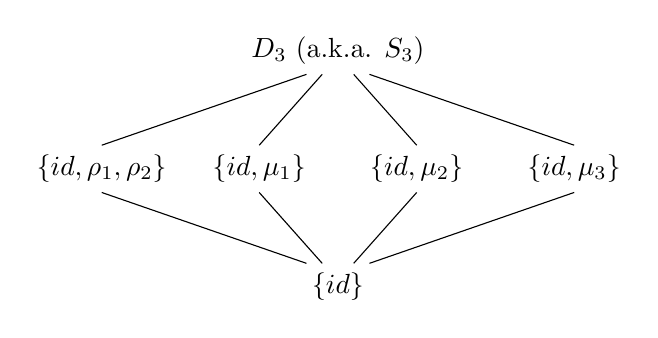
\begin{tikzpicture}[scale=1]

\draw  (0,0.3) -- (2.6,1.2);
\draw  (2,0.3) -- (2.8,1.2);
\draw  (4,0.3) -- (3.2,1.2);
\draw  (6,0.3) -- (3.4,1.2);

\draw  (0,-0.3) -- (2.6,-1.2);
\draw  (2,-0.3) -- (2.8,-1.2);
\draw  (4,-0.3) -- (3.2,-1.2);
\draw  (6,-0.3) -- (3.4,-1.2);

\node at (0, 0) {$\{{\var  id}, \rho_1, \rho_2\}$};
\node at (2, 0) {$\{{\var  id}, \mu_1\}$};
\node at (4, 0) {$\{  {\var  id}, \mu_2 \}$};
\node at (6, 0) {$\{  {\var  id}, \mu_3 \}$};
\node at (3, 1.5) {$D_3$ (a.k.a. $S_3$)};
\node at (3,-1.5) {$\{ {\var  id} \}$};
\end{tikzpicture}
\end{center}
\caption{Subgroups of $D_3 (a.k.a. S_3)$}
\label{subgrpsS3}
\end{figure}

Although not every group  (and not every subgroup) is cyclic, we may use cyclic subgroups to help us
enumerate all possible subgroups of a given group, with the benefit of the following result:

\begin{prop}{orbit_sgp}
Given a group $G$ and a subgroup $H \subset G$, and suppose that $a \in H$.  Then $\langle a \rangle \subset H$.
\end{prop}

\begin{exercise}{prove_orbit_sgp}
Prove Proposition~\ref{proposition:groups:orbit_sgp}
\end{exercise}

Proposition~\ref{proposition:groups:orbit_sgp} makes it much easier to find subgroups of a given group, because it greatly cuts down
on the possibilities.

\begin{example}{S3_subgroups}
We showed in Example~\ref{example:groups:Not_Cyclic_S3} that $D_3$ has 4 cyclic subgroups, and that every element of $D_3$ is in at least one of these subgroups.  Proposition~\ref{proposition:groups:orbit_sgp} shows that, for example, any subgroup containing $\rho_1$ must also contain $id$ and  $\rho_2$, since $\langle \rho_1 \rangle = \{id, \rho_1, \rho_2\}$.  Let's try to find a larger subgroup $H \subset D_3$ that contains $\rho_1$.  If we add any other element  (which must be  $\mu_k$ for some $k=1,2$ or $3$), then we must also add $\rho_1 \mu_k$ and $\rho_2 \mu_k$, which means that $H$ contains  all 6 elements of $D_3$. It follows that $H=D_3$. Similarly, if we try to find a subgroup $K$ that contains $\mu_k$ by adding another reflection $\mu_j (j \neq k)$, we find that $\mu_j \mu_k$ and $\mu_j \mu_k$  must also be in $K$, which means that $\rho_1$ must also be in $K$. But we've just finished shown that if $\rho_1 \in K$ and $\mu_k \in K$, then  $K=G$.  It follows that the only proper nontrivial subgroups of $D_3$ are the four cyclic subgroups shown in Figure~\ref{subgrpsS3}.
\end{example}

\begin{exercise}{d_4subgroups}
\begin{enumerate}[(a)]
\item
Find all cyclic subgroups of  the symmetry group of the square (i.e. $D_4$)  by finding $\langle a \rangle$ for every element $a \in D_4$.
\item
Find all nontrivial proper subgroups of $D_4$  (You may follow the procedure used in Example~\ref{example:groups:S3_subgroups} if you wish.) 
\item
Show that at least one of the subgroups in (a)  is abelian and not cyclic.
\end{enumerate}
\end{exercise}      

It is not true that every abelian group is cyclic (see Exercise~\ref{exercise:groups:d_4subgroups}.  However, we can prove the converse, namely:
 
\begin{prop}{cyclic_abelian}
Every cyclic group is abelian.
\end{prop}
 
 
\begin{proof}
Let $G$ be a cyclic group and $a \in G$ be a generator for $G$. If
$g$ and $h$ are in $G$, then they can be written as powers of $a$,
say $g = a^r$ and $h = a^s$. It follows that
\[
g  h = a^r a^s = a^{r+s} = a^{s+r} = a^s a^r = h g.
\]
Since $g$ and $h$ were arbitrary elements of $G$, it follows that $G$ is abelian.
\end{proof}
 
How about the converse of Proposition~\ref{proposition:groups:cyclic_abelian}? Is it true that every abelian group is cyclic? As it turns out, No. The following proposition gives an example:

\begin{prop}{realNotCyclic}
The group $({\mathbb R},+)$ is not cyclic.
\end{prop}

\begin{proof}
We'll use our old workhorse, proof by contradiction.  Suppose that $a$ is a generator of $\mathbb{R}$, i.e. $\langle a \rangle = \mathbb{R}$.  Then since $a/2 \in  \mathbb{R}$, it follows that  $a/2 \in \langle a \rangle$. This means $a/2 =ka$ for some integer k.  Rearranging this equation, we find that $a(1/2-k)=0$.  By the zero-divisor property of real numbers, this implies that either $a=0$ or $1/2-k = 0$ (or both). But $a$ cannot be 0, because $\langle 0 \rangle = 0$.  Also, $1/2-k \neq 0$, since $k$ is an integer.  This contradiction shows that  our assumption that ${\mathbb R} = \langle a \rangle$ is false. Therefore ${\mathbb R} \neq \langle a \rangle$ for any real number $a$, and ${\mathbb R}$ is not cyclic.
\end{proof}

\begin{exercise}{not_cyclic}
\begin{enumerate}[(a)]
\item
Show that ${\mathbb Q}$ is not cyclic.   
\item
Show that ${\mathbb C}$ is not cyclic.
\end{enumerate}
\end{exercise}
 
%%%Back in Section~\ref{Examples} we defined the \term*{product of groups}\index{Product!of groups} (see Definition~\ref{def:ProductOfGroups}).  The product of groups $G$ and $H$ is denoted by $G \times H$) and consists of pairs $\left\{(g,h), g \in G, h \in H \right\}$.The group operation on $G \times H$ is defined by $ (g_1, h_1) \circ (g_2, h_2) := (g_1g_2, h_1h_2),$
%%%where $g_1g_2$ uses the group operation in $G$ and $h_1h_2$ uses the group operation in $H$.



  
\subsection{Subgroups of cyclic groups}
 
 
We can ask some interesting questions about cyclic subgroups of a
group and subgroups of a cyclic group.  If $G$ is a group, which
subgroups of $G$ are cyclic? If $G$ is a cyclic group, what type of
subgroups does $G$ possess? 
 
 
 
\begin{prop}{}
Every subgroup of a cyclic group is cyclic.
\end{prop}
 
 
\begin{proof}
The main tools used in this proof are the division algorithm, which we mentioned in Proposition~\ref{proposition:modular:DivAlg},  and the
Principle of Well-Ordering, which we mentioned in Section~\ref{subsec:orderprop}.
 
Let $G$ be a cyclic group generated by $a$
and suppose that $H$ is a subgroup of $G$. If $H = \{ e \}$, then
trivially $H$ is cyclic. Suppose that $H$ contains some other element
$g$ distinct from the identity. Then $g$ can be written as
$a^n$ for some integer $n$. We can assume that $n > 0$.  
 Define the set $S$ by:  $S = \{j \in \mathbb{N} \text{ such that } a^j=g\}$. We have just shown that $S$ is nonempty. The Principle of Well-Ordering tells us that any nonempty subset of the natural numbers has  a smallest element.  Let $m$ be the smallest element of $S$.

We claim that $h = a^m$ is a generator for $H$.  We must show that
every $h' \in H$ can be written as a power of $h$. Since $h' \in H$
and $H$ is a subgroup of $G$, $h' = a^k$ for some positive integer
$k$. Using the division algorithm, we can find numbers $q$ and $r$
such that $k = mq +r$ where $0 \leq r < m$; hence,
\[
a^k = a^{mq +r} = (a^m)^q a^r = h^q a^r.
\]
So we can solve for $a^r$:  $a^r =h^{-q}  a^k $. Since $a^k$ and $h^{-q}$ are in $H$, $a^r$ must
also be in $H$.  However, $m$ was the smallest positive number such that
$a^m$ was in $H$; consequently, $r=0$ and so $k=mq$. Therefore, 
\[
h' = a^k = a^{mq} =  h^q
\]
and $H$ is generated by $h$.
\end{proof}
 
 
\begin{prop}{nZ_sgp}
The subgroups of ${\mathbb Z}$ are exactly $n{\mathbb Z}$ for $n = 0, 1, 2,
\ldots$. 
\end{prop}

\begin{exercise}{}
Prove Proposition~\ref{proposition:groups:nZ_sgp}
\end{exercise}

\begin{exercise}{}
Let $H = \{2^k : k \in {\mathbb Z} \}$. We know that $H$ is a subgroup of $\mathbb{Q}$.  Find all subgroups of $H$. 
\end{exercise}
 
 
\begin{prop}{Cyclic_subgrp_order}
Let $G$ be a cyclic group of order $n$ and suppose that $a$ is a
generator for  $G$. Then $a^k=e$ if and only if $n$ divides $k$.
\end{prop}
 
 
\begin{proof}
Since $G=\langle a \rangle$ it follows from Proposition~\ref{proposition:groups:OrderEltCyclic} that $|a|=n$. In Exercise~\ref{exercise:groups:OrderEltCyclic} (a) we proved that  $a^k =  a^{\bmod(m,n)}$. Let $r =\bmod(m,n)$.  If $r=0$ (which is the same thing as saying that $n$ divides $k$) this implies $a^k =  a^{0} = e$. Otherwise, if it must be the case that $0< r< n=|a|$, and by the definition of $|a|$ it follows that $a^r \neq e$. This concludes the proof.
\end{proof}

\begin{prop}{}
Let $G$ be a cyclic group of order $n$ and suppose that $a \in G$ is a
generator of the group.  If $b = a^k$, then the order of $b$ is $n
/d$, where $d = \text{gcd}(k,n)$. 
\end{prop}
 
 
\begin{proof}
We wish to find the smallest integer $m$ such that $e = b^m = a^{km}$.
By Proposition~\ref{proposition:groups:Cyclic_subgrp_order}, this is the smallest integer $m$ such that
$n$ divides $km$ or, equivalently, $n/d$ divides $m(k/d)$. (Note that $n/d$ and $k/d$ are both integers, since $d$ divides both $n$ and $k$.)  Since $d$ is
the greatest common divisor of $n$ and $k$, $n/d$ and $k/d$ are
relatively prime. Hence, for $n/d$ to divide $m(k/d)$ it must divide
$m$.  The smallest such $m$ is $n/d$. 
\end{proof}
 
 
\begin{corollary}
The generators of ${\mathbb Z}_n$ are the integers $r$ such that $1 \leq
r < n$ and $\text{gcd}(r,n) =  1$. 
\end{corollary}
 
 
\begin{example}{Cyclic_Z16}
Let us examine the group ${\mathbb Z}_{16}$.  The numbers 1, 3, 5, 7, 9,
11, 13, and 15 are the elements of ${\mathbb Z}_{16}$ that are relatively
prime to 16.  Each of these elements generates ${\mathbb Z}_{16}$. For
example, 9 is a generator because:
\begin{alignat*}{3}
1 \cdot 9  & =  9  & \qquad 2 \cdot 9  & = 2  & \qquad 3 \cdot 9  & = 11 \\
4 \cdot 9  & =  4  & \qquad 5 \cdot 9  & = 13 & \qquad	6 \cdot 9 & = 6  \\
7 \cdot 9  & =  15 & \qquad 8 \cdot 9  & = 8  & \qquad	9 \cdot 9 &  = 1  \\
10 \cdot 9 & =  10 & \qquad 11 \cdot 9 & = 3  & \qquad	12 \cdot 9 &  = 12 \\
13 \cdot 9 & =  5 &  \qquad 14 \cdot 9 & = 14 &  \qquad	15 \cdot 9 & = 7.
\end{alignat*}
\end{example}



\markright{EXERCISES}
\section{Additional group and subgroup exercises}\label{sec:addGpEx}


\begin{exercise}{} 
Write out Cayley tables for groups formed by the symmetries of a
rectangle and for $({\mathbb Z}_4, +)$. How many elements are in each
group? Are the groups the same? Why or why not? 
\end{exercise} 
 
\begin{exercise}{} 
Describe the symmetries of a rhombus and prove that the set of
symmetries forms a group. Give Cayley tables for both the symmetries
of a rectangle and the symmetries of a rhombus. Are the symmetries of
a rectangle and those of a rhombus the same?
\end{exercise} 
 
\begin{exercise}{} 
Give a multiplication table for the group $U(12)$.
\end{exercise} 
 
  
\begin{exercise}{} 
Prove that the set of matrices of the form
\[
\begin{pmatrix}
1 & x & y \\
0 & 1 & z \\
0 & 0 & 1
\end{pmatrix}
\]
where $x,y,z \in \mathbb{C}$ is a group under matrix multiplication.  This group, known as the
\term{Heisenberg group},\index{Group!Heisenberg} is important in
quantum physics.
\end{exercise}  
%Matrix multiplication in the Heisenberg group is
%defined by  
%\[
%\begin{pmatrix}
%1 & x & y \\
%0 & 1 & z \\
%0 & 0 & 1
%\end{pmatrix}
%\begin{pmatrix}
%1 & x' & y' \\
%0 & 1 & z' \\
%0 & 0 & 1
%\end{pmatrix}
%=
%\begin{pmatrix}
%1 & x+x' & y+y'+xz' \\
%0 & 1 & z+z' \\
%0 & 0 & 1
%\end{pmatrix}.
%\]
  

\begin{exercise}{}\label{ex:groups:quat}
List all subgroups of the quaternion group $Q_8$. \hyperref[sec:groups:hints]{(*Hint*)}
\end{exercise} 
 
\begin{exercise}{}
Prove or disprove: $SL_2( {\mathbb Z} )$, the set of $2 \times 2$
matrices with integer entries and determinant one, is a subgroup of
$SL_2( {\mathbb R} )$. 
\end{exercise}
 
\begin{exercise}{}\label{ex:eoc:31}
Prove that the intersection of two subgroups of a group $G$ is also a
subgroup of $G$. 
 \end{exercise}
 
\begin{exercise}{}
Prove or disprove:  If $H$ and $K$ are subgroups of a group $G$, then
$H \cup K$ is a subgroup of $G$. 
\end{exercise} 
 
\begin{exercise}{}
Prove or disprove: If $H$ and $K$ are subgroups of a group $G$, then
$H K = \{hk : h \in H \text{ and } k \in K \}$ is a subgroup of $G$.
What if $G$ is abelian? 
\end{exercise} 
 
\begin{exercise}{}
Let $G$ be a group. Show that
\[
Z(G) = \{ x \in G : gx = xg \mbox{ for all $g \in G$}
\}\label{centerofagroup} 
\]
is a subgroup of $G$. This subgroup is called the \term{
center}\index{Center!of a group} of $G$. 
\end{exercise} 
 
 
\begin{exercise}{}
Give an example of an infinite group in which every nontrivial
subgroup is infinite.
\end{exercise}
 
\begin{exercise}{}
Prove or disprove: Every nontrivial subgroup of an non-abelian group is
non-abelian.
\end{exercise}  

\begin{exercise}{}\label{ex:eoc:11}
\begin{enumerate}[(a)]
\item
Recall the discussion of Section~\ref{sec:miracle}, which explains how two apparently different groups can in fact be essentially the ``same" group. Find two groups of order eight that we have studied are not the ``same'' in this sense, and explain why they can't be considered as examples of the ``same'' group.  
\item
Using the previous exercise (which introduces ${\mathbb Z}_2^n$), give an example of a third group that is not the ``same'' as the two groups you found in (a), and explain why it is not the ``same''.
\end{enumerate}
\end{exercise}
 
\begin{exercise}{}
Give a specific example of some group $G$ and elements $g, h \in G$
where $(gh)^n \neq g^nh^n$, for some natural number $n$. 
\end{exercise} 
 

  
\begin{exercise}{}
Let $a$ and $b$ be elements in a group $G$.  Prove that $ab^na^{-1} =
(aba^{-1})^n$. 
\end{exercise}

\begin{exercise}{}\label{ex:eoc:15}
Given a group $G$ which includes elements $g_1,\ldots g_n$. Prove that the inverse of $g _1 g_2 \cdots g_n$ is $g_n^{-1}
g_{n-1}^{-1} \cdots g_1^{-1}$. 
\end{exercise} 
 
\begin{exercise}{}
Let $U(n)$ be the group of units in ${\mathbb Z}_n$. If $n>2$, prove that
there is an element $k \in U(n)$ such that $k^2 = 1$ and $k \neq 1$.
\end{exercise}
 
\begin{exercise}{}\label{ex:eoc:evenInv}
Show that if $G$ is a finite group of even order, then there is an $a
\in G$ such that $a$ is not the identity and $a^2 = e$.
\hyperref[sec:groups:hints]{(*Hint*)} 
\end{exercise} 
 
 
%\item
%Prove the right and left cancellation laws for a group $G$; that is,
%show that in the group $G$, $ba = ca$ implies $b = c$ and $ab = ac$
%implies $b = c$ for elements $a, b, c \in G$.  
 

\begin{exercise}{}\label{ex:eoc:abelian1}
Let $G$ be a group and suppose that $(ab)^2 = a^2b^2$ for all $a$ and
$b$ in $G$.  Prove that $G$ is an abelian group.
\hyperref[sec:groups:hints]{(*Hint*)}  
\end{exercise}

\begin{exercise}{}\label{ex:eoc:abelian2}
Show that if $a^2 = e$ for all $a \in G$, then $G$ must be an abelian group. 
\hyperref[sec:groups:hints]{(*Hint*)} 
\end{exercise}
 
\begin{exercise}{}\label{ex:groups:2elt}
If $(xy)^2 = xy$ for all $x$ and $y$ in $G \setminus {e}$, prove that $G$ must be
abelian.
\hyperref[sec:groups:hints]{(*Hint*)}
\end{exercise}

\begin{exercise}{}\label{ex:groups:abelian_proof}
If $xy = x^{-1} y^{-1}$ for all $x$ and $y$ in $G \setminus {e}$, prove that $G$
must be abelian.
\end{exercise} 
 
\begin{exercise}{}
Let $H$ be a subgroup of $G$ and
\[
N(H) = \{ g \in G : gh = hg \mbox{ for all $h \in H$}  \}.
\]
Prove $N(H)$ is a subgroup of $G$.  This subgroup is called the \term{
normalizer}\index{Normalizer} of $H$ in $G$. 
\end{exercise}
 
